\documentclass[english]{tudscrreprt}
\usepackage{babel}
\usepackage{iftex}
\iftutex
  \usepackage{fontspec}
\else
  \usepackage[T1]{fontenc}
  \usepackage[english=english]{hyphsubst}
\fi
\usepackage{scrhack}
\usepackage{tudscrsupervisor}

\AfterPackage*{hyperref}{%
\usepackage[%
  acronym,% Abbreviations
  symbols,% Mathematical symbols
  nomain,% No main glossary
  nogroupskip,%
  toc,%
  section=chapter,%
  nostyles,%
  translate=babel,%
% Easy to use with Tex Live
  xindy={language=english},
]{glossaries}
\makeglossaries
}% End of AfterPackage

\AfterPackage*{glossaries}{%
\newglossarystyle{acrotabu}{%
  \renewenvironment{theglossary}{%
    \begin{tabu}{@{}lX<{\strut}l@{}}% 'spread 0pt' defekt in v2.9
  }{%
    \end{tabu}\par\bigskip%
  }%
  \renewcommand*{\glossaryheader}{}%
  \renewcommand*{\glsgroupheading}[1]{}%
  \renewcommand*{\glsgroupskip}{}%
  \renewcommand*{\glossentry}[2]{%
    \glsentryitem{##1}% Entry number if required
    \glstarget{##1}{\sffamily\bfseries\glossentryname{##1}} &
    \glsentrydesc{##1} &
    ##2\tabularnewline
  }
}

\newcommand*{\newformulasymbol}[5][]{%
  \newglossaryentry{#2}{%
    type=symbols,%
    name={#3},%
    description={\nopostdesc},%
    symbol={\ensuremath{#4}},%
    user1={\ensuremath{\mathrm{#5}}},%
    sort={#2},%
    #1%
  }%
}

\defglsentryfmt[symbols]{%
  \ifmmode%
    \glssymbol{\glslabel}%
  \else%
    \glsgenentryfmt~\glsentrysymbol{\glslabel}%
  \fi%
}
\newglossarystyle{symblongtabu}{%
  \renewenvironment{theglossary}{%
    \begin{longtabu}[l]{ccX<{\strut}l}% 'spread 0pt' defekt in v2.9
  }{%
    \end{longtabu}%
  }%
  \renewcommand*{\glsgroupheading}[1]{}%
  \renewcommand*{\glsgroupskip}{}%
  \renewcommand*{\glossaryheader}{%
    \toprule
    \bfseries Symbol & \bfseries Unit &
    \bfseries Description & \bfseries Page(s)
    \tabularnewline\midrule\endhead%
    \bottomrule\endfoot%
  }%
  \renewcommand*{\glossentry}[2]{%
    \glsentryitem{##1}% Entry number if required
    \glstarget{##1}{\glossentrysymbol{##1}} &
    \glsentryuseri{##1} &
    \glossentryname{##1} &
    ##2\tabularnewline%
  }%
}
}% End of AfterPackage

\usepackage{csquotes}
\usepackage[backend=biber,style=alphabetic]{biblatex}
\usepackage{graphicx}
\usepackage{subcaption}

\usepackage{floatrow}
\usepackage{xcolor}
\usepackage{listings}


% Listings configuration for algorithm display
\lstset{
    basicstyle=\ttfamily\small,
    frame=single,
    numbers=left,
    numberstyle=\tiny,
    breaklines=true,
    showstringspaces=false,
    commentstyle=\color{gray},
    keywordstyle=\color{blue},
    stringstyle=\color{red},
    backgroundcolor=\color{gray!10},
    captionpos=b
}

\usepackage{filecontents}
\begin{filecontents}{\jobname-temp.bib}
@article{garg1997,
  author    = {Garg, Naveen and Vazirani, Vijay V. and Yannakakis, Mihalis},
  title     = {Primal-dual approximation algorithms for integral flow and multicut in trees},
  journal   = {Algorithmica},
  volume    = {18},
  number    = {1},
  pages     = {3--20},
  year      = {1997},
  publisher = {Springer},
  language  = {english},
}
@article{calinescu2000,
  author    = {Calinescu, Gruia and Karloff, Howard and Rabani, Yuval},
  title     = {An improved approximation algorithm for {MULTICUT}},
  journal   = {Journal of Computer and System Sciences},
  volume    = {60},
  number    = {3},
  pages     = {564--574},
  year      = {2000},
  publisher = {Elsevier},
  language  = {english},
}
@book{schrijver2003,
  author    = {Schrijver, Alexander},
  title     = {Combinatorial Optimization: Polyhedra and Efficiency},
  volume    = {A},
  series    = {Algorithms and Combinatorics},
  publisher = {Springer-Verlag},
  address   = {Berlin},
  year      = {2003},
  language  = {english},
}
@article{gupta2004,
  author    = {Gupta, Anupam and Hajiaghayi, MohammadTaghi and R\"{a}cke, Harald},
  title     = {Oblivious network design},
  journal   = {Proceedings of the 36th Annual ACM Symposium on Theory of Computing},
  pages     = {383--392},
  year      = {2004},
  publisher = {ACM},
  language  = {english},
}

@manual{unity2023,
  author    = {Unity Technologies},
  title     = {Unity Game Engine Documentation},
  year      = {2023},
  url       = {https://docs.unity3d.com/},
  language  = {english},
}
@manual{gurobi2023,
  author    = {Gurobi Optimization, LLC},
  title     = {Gurobi Optimizer Reference Manual},
  year      = {2023},
  url       = {https://www.gurobi.com/documentation/},
  language  = {english},
}
@article{poisson2007,
  author    = {Bridson, Robert},
  title     = {Fast Poisson disk sampling in arbitrary dimensions},
  journal   = {ACM SIGGRAPH 2007 sketches},
  pages     = {22},
  year      = {2007},
  publisher = {ACM},
  language  = {english},
}
@article{delaunay1934,
  author    = {Delaunay, Boris},
  title     = {Sur la sphère vide},
  journal   = {Bulletin de l'Académie des Sciences de l'URSS},
  volume    = {6},
  pages     = {793--800},
  year      = {1934},
  language  = {french},
}
@article{bansal2004,
  author    = {Bansal, Nikhil and Blum, Avrim and Chawla, Shuchi},
  title     = {Correlation clustering},
  journal   = {Machine Learning},
  volume    = {56},
  number    = {1-3},
  pages     = {89--113},
  year      = {2004},
  publisher = {Springer},
  language  = {english},
}
@article{demaine2006,
  author    = {Demaine, Erik D. and Emanuel, Dotan and Fiat, Amos and Immorlica, Nicole},
  title     = {Correlation clustering in general weighted graphs},
  journal   = {Theoretical Computer Science},
  volume    = {361},
  number    = {2-3},
  pages     = {172--187},
  year      = {2006},
  publisher = {Elsevier},
  language  = {english},
}
@article{charikar2005,
  author    = {Charikar, Moses and Guruswami, Venkatesan and Wirth, Anthony},
  title     = {Clustering with qualitative information},
  journal   = {Journal of Computer and System Sciences},
  volume    = {71},
  number    = {3},
  pages     = {360--383},
  year      = {2005},
  publisher = {Elsevier},
  language  = {english},
}
@article{andres2012a,
  author    = {Andres, Björn and Kappes, Jörg Hendrik and Beier, Thorsten and Köthe, Ullrich and Hamprecht, Fred A.},
  title     = {Probabilistic image segmentation with closedness constraints},
  journal   = {2011 International Conference on Computer Vision},
  pages     = {2611--2618},
  year      = {2012},
  publisher = {IEEE},
  language  = {english},
}
@article{andres2012b,
  author    = {Andres, Björn and Kröger, Thorsten and Briggman, Kevin L. and Denk, Winfried and Korogod, Natalya and Knott, Graham and Koethe, Ullrich and Hamprecht, Fred A.},
  title     = {Globally optimal closed-surface segmentation for connectomics},
  journal   = {European Conference on Computer Vision},
  pages     = {778--791},
  year      = {2012},
  publisher = {Springer},
  language  = {english},
}

@misc{fantasyhextiles,
  author    = {The Clover Patch},
  title     = {Fantasy Hex Tiles},
  year      = {2017},
  url       = {https://cuddlyclover.itch.io/fantasy-hex-tiles},
  note      = {Free asset pack under Creative Commons Attribution v4.0 International license}
}
\end{filecontents}
\addbibresource{\jobname-temp.bib}

\usepackage{caption}
\captionsetup{font=sf,labelfont=bf,labelsep=space}
\usepackage{floatrow}
\floatsetup{font=sf}
\floatsetup[table]{style=plaintop}
\captionsetup{singlelinecheck=off,format=hang,justification=raggedright}
\DeclareCaptionSubType[alph]{figure}
\DeclareCaptionSubType[alph]{table}
\captionsetup[subfloat]{labelformat=brace,list=off}

\usepackage{booktabs}
\usepackage{array}
\usepackage{tabularx}
\usepackage{tabulary}
\usepackage{tabu}
\usepackage{longtable}

\usepackage{quoting}

\usepackage[babel]{microtype}

\usepackage{enumitem}
\setlist[itemize]{noitemsep}

\usepackage{ellipsis}
\let\ellipsispunctuation\relax

\usepackage{xfrac}

\usepackage{isodate}

\usepackage[colorlinks,linkcolor=blue]{hyperref}

\begin{document}

\faculty{Faculty of Computer Science}
\title{%
  Multicut Game: Alliance Divider
}
\thesis{research}
\graduation{Research Project}
\renewcommand{\graduationtext}{}
\author{%
  Sheng, Yichao%
  \matriculationnumber{5171752}%
  % \dateofbirth{1.1.1995}%
  % \placeofbirth{Beijing}%
  % \course{Computer Science}%
  % \discipline{Algorithmic Game Theory}%
}
\matriculationyear{2023}
\supervisor{Jannik Irmai}
\professor{Prof. Dr. Bjoern Andres}
\date{12.08.2025}
\issuedate{07.04.2025}
\duedate{12.08.2025}
\makecover
\maketitle

\newcommand{\taskcontent}{%
  The Multicut Game project aims to transform the complex combinatorial optimization
  problem of graph partitioning into an engaging educational game experience.
  The project focuses on developing an interactive game called "Alliance Divider" that teaches players
  about the Multicut Problem while providing an optimal solution using Integer
  Linear Programming (ILP) with Gurobi solver.

  The main objectives include creating an intuitive game interface that
  represents city-states as nodes and their relationships as weighted edges,
  implementing the core gameplay mechanics of cutting hostile ties while
  preserving friendly alliances, and developing a robust technical architecture
  that bridges Unity game engine with Python optimization algorithms.
}


\TUDoption{abstract}{section}
\begin{abstract}
  This thesis presents "Alliance Divider", an educational game that transforms the complex Multicut Problem from combinatorial optimization into an engaging interactive experience. The project addresses the challenge students face in understanding complex algorithmic concepts without prior computational background.

  The game enables players to learn graph theory and optimization principles by cutting hostile connections and preserving friendly alliances between city-states in a medieval political setting. The core objective is to create an educational tool that helps students understand the Multicut Problem and experience NP-hard computational complexity through hands-on problem-solving, while maintaining mathematical rigor.

  The project demonstrates successful gamification through Unity-Python integration and Integer Linear Programming optimization using the Gurobi solver. Performance optimizations include selective territory coloring with caching mechanisms that reduce computational overhead by up to 60\%.

  The main contribution lies in successfully integrating the Multicut algorithm into a game environment without distorting its mathematical essence, demonstrating practical applications in social network analysis, and making mathematical concepts more memorable through interactive gameplay.
\end{abstract}



\tableofcontents
\listoffigures
\listoftables

% moved printing of acronyms/symbols to after their definitions

\chapter{Acronyms and Mathematical Notation}

\section{Acronyms}
\newacronym{ilp}{ILP}{Integer Linear Programming}
\newacronym{np}{NP}{Non-deterministic Polynomial time}
\newacronym{api}{API}{Application Programming Interface}
\newacronym{json}{JSON}{JavaScript Object Notation}
\newacronym{hud}{HUD}{Heads-Up Display}
\newacronym{ui}{UI}{User Interface}

In the context of the Multicut Game project, several key acronyms are used throughout
this document. The \gls{ilp} approach is central to solving the optimization
problems, while \gls{np}-hard complexity characterizes the computational
challenge. The game's \gls{ui} and \gls{hud} provide intuitive interaction,
while \gls{api} and \gls{json} facilitate cross-language communication.

\section{Mathematical Symbols}
\newformulasymbol{G}{Graph}{G}{(V,E)}
\newformulasymbol{V}{Vertex Set}{V}{}
\newformulasymbol{E}{Edge Set}{E}{}
\newformulasymbol{w}{Edge Weight}{w}{}
\newformulasymbol{C}{Cut Set}{C}{}
\newformulasymbol{c}{Cut Cost}{c}{}

The mathematical foundation of the Multicut Game project is based on graph theory,
where \gls{G} represents the game's network structure with vertex set \gls{V}
representing city-states and edge set \gls{E} representing relationships.
Each edge has an associated weight \gls{w} representing the cost of cutting
that relationship. The objective is to find a cut set \gls{C} that minimizes
the total cut cost \gls{c} while satisfying the cycle inequality constraints.

\newformulasymbol{q}{Hexagonal Axial Coordinate}{q}{}
\newformulasymbol{r}{Hexagonal Axial Coordinate}{r}{}
\newformulasymbol{hexSize}{Hexagonal Grid Size}{hexSize}{}

\printacronyms[style=acrotabu]
\printsymbols[style=symblongtabu]

\chapter{Introduction}

This chapter introduces the Multicut Game project and its objectives. The project addresses a fundamental challenge in computer science education: the difficulty students face in understanding complex algorithmic concepts without prior computational background. Through extensive investigation, it was found that traditional teaching methods often fail to engage students effectively when introducing advanced topics such as the Multicut Problem, a crucial concept in combinatorial optimization and graph theory.

The project aims to transform the complex combinatorial optimization problem of graph partitioning into an engaging educational game experience that serves as both an effective learning tool and an entertaining puzzle game. The primary motivation stems from the recognition that the Multicut Problem holds significant importance in algorithm courses, yet students struggle to grasp its theoretical foundations and practical applications through conventional teaching approaches.

The core objective is to create an educational game that enables students to understand what the Multicut Problem is and experience the computational complexity of NP-hard problems through hands-on problem-solving, while maintaining the mathematical rigor of the original algorithm. The game achieves this through infinite level generation, three distinct difficulty levels (Easy, Medium, Hard), and an intuitive political strategy theme that makes abstract mathematical concepts accessible and memorable.

The project's main contribution lies in successfully integrating the Multicut algorithm into a game environment without distorting its mathematical essence, demonstrating the algorithm's practical applications and making the underlying mathematical concepts more memorable through interactive gameplay. The following chapters will provide detailed analysis of the mathematical foundations, game design, technical implementation, and evaluation of the Alliance Divider game.

\chapter{Background and Related Work}

\section{The Multicut Problem}
The multicut problem is a fundamental concept in combinatorial optimization and graph theory that was first studied in the late 20th century \cite{bansal2004}. It involves partitioning a graph into multiple components by cutting edges while minimizing the total cost of the cuts. This problem has significant applications in various fields including computer vision, network design, and social network analysis.

Let $G = (V, E)$ be an undirected graph. A set of edges $M \subseteq E$ is called a multicut of $G$ if and only if for every cycle $C = (V_C, E_C)$ in $G$, it holds that $|M \cap E_C| \ne 1$. That is, no cycle contains exactly one edge from $M$.

The set of all multicuts of $G$ is denoted by $\mathcal{M}(G)$. The multicut problem is the following optimization problem:

\[
\min_{M \in \mathcal{M}(G)} \sum_{e \in M} c_e
\]

where $c_e$ represents the cost of cutting edge $e$.

\begin{figure}[h]
\centering
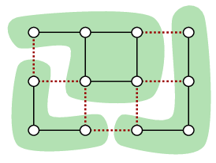
\includegraphics[width=0.3\textwidth]{figures/multicut.png}
\caption{Multicut problem example: A 3×4 grid graph showing cut edges (red dashed lines) and partitioned regions (light green areas). This example demonstrates the cycle inequality constraint.}
\label{fig:multicut_example}
\end{figure}

The mathematical formulation of the multicut problem provides the foundation for understanding its computational complexity and solution approaches. As illustrated in Figure~\ref{fig:multicut_example}, the problem involves cutting edges to partition the graph while satisfying the cycle inequality constraints. The problem is NP-hard \cite{demaine2006}, meaning that finding optimal solutions for large instances is computationally challenging. However, this complexity makes it an excellent candidate for educational gamification, as it demonstrates real-world algorithmic challenges that students can experience firsthand.

The problem's applications span multiple domains, from image segmentation in computer vision \cite{andres2012a} to community detection in social networks \cite{charikar2005}. This broad applicability makes it an ideal subject for educational games, as students can see how abstract mathematical concepts translate into practical problem-solving scenarios. The multicut problem is also known as "correlation clustering" and "coalition structure generation" in different contexts, demonstrating its versatility across various research domains.

\subsection{Social Network Analysis Application}
The Alliance Divider game is specifically inspired by the social network analysis applications of the Multicut Problem. In social network analysis, the problem is used to identify communities and clusters within complex networks by analyzing relationships between entities. The game translates this concept into a medieval political setting where city-states represent network nodes and their relationships represent weighted edges.

The complexity of political relationships in the game mirrors real-world social networks, where entities may have conflicting interests and complex alliance dynamics. Just as social network analysis seeks to understand community formation and relationship patterns, the game challenges players to analyze complex political landscapes and identify optimal alliance formations. This application demonstrates how the Multicut Problem can be used to model and solve real-world relationship optimization challenges, making the mathematical concept more tangible and relatable to students.

\section{Academic Gamification}
The concept of transforming complex mathematical problems into engaging games has been successfully demonstrated by various applications. Notable examples include Flow Free, 2048, and Sudoku, which have established stable audiences and demonstrated consistent market performance as puzzle games. These games demonstrate how mathematical concepts can be effectively gamified while maintaining their intellectual challenge and educational value.

Flow Free specifically demonstrates how graph connectivity problems can be transformed into intuitive puzzle mechanics, achieving over 100 million downloads since its 2012 release. The game's success lies in its ability to teach players about graph theory concepts through intuitive gameplay without losing the core algorithmic complexity. This provides a valuable model for the Alliance Divider project, showing that mathematical problems can be successfully gamified while maintaining educational rigor.

The stable market performance of these puzzle games indicates a consistent demand for intellectually challenging games that combine entertainment with educational value, supporting the viability of educational algorithm games as a genre.

\chapter{Game Design and Implementation}

\section{Game Design Documentation}

\subsection{Working Title}
\textbf{Alliance Divider: Cut the Enemies, Unite the Allies}

The title communicates the core gameplay mechanic (cutting connections) and the strategic objective (forming alliances), while emphasizing the political strategy theme.

\subsection{Current Status}
The game has been fully developed with all core mechanics implemented and functional. The project has been completed successfully, achieving all major milestones including the complete implementation and testing of core gameplay mechanics, successful completion of the Unity-Python integration architecture, operational ILP solver integration with Gurobi, functional user interface and HUD systems, and implementation of level progression systems. The game is now ready for educational use and further development.

\subsection{Concept Statement}
A political strategy puzzle game where players act as royal strategists, cutting hostile connections between city-states while preserving friendly alliances to form stable political networks.

\subsection{Genre}
Alliance Divider is classified as an Educational Strategy Puzzle Game that combines three distinct elements: political strategy for decision-making based on relationship dynamics, graph theory puzzle mechanics for mathematical problem-solving through edge cutting, and educational game design for learning combinatorial optimization concepts.

\subsection{Target Audience}
Primary: Computer science students and researchers (ages 18-35)
Secondary: Mathematics enthusiasts and puzzle game players
Educational Focus: Undergraduate and graduate level algorithm courses
ESRB Rating: E (Everyone) - No violence, suitable for all ages

\subsection{Concept Paragraph and Unique Selling Points}
Alliance Divider transforms the complex Multicut Problem from combinatorial optimization into an intuitive political strategy game. Players manage relationships between city-states, making strategic decisions about which connections to sever to achieve optimal alliance formations.

The game's unique selling points distinguish it from existing educational games. First, it represents the first successful attempt to make the Multicut Problem accessible through intuitive political strategy mechanics, achieving mathematical gamification without sacrificing theoretical rigor. Second, the real-time optimization feature provides live ILP solver integration that delivers instant optimal solutions and educational feedback. Third, the innovative cross-language architecture demonstrates modern game development techniques through Unity-Python integration. Fourth, the game maintains educational depth by preserving mathematical rigor while providing engaging gameplay. Finally, the sophisticated territory coloring system ensures visual clarity, making complex graph partitions immediately understandable to players.

\subsection{Player Experience}
\textbf{Player Role:} Royal Strategist analyzing political networks in a medieval fantasy setting

\textbf{Setting:} Multiple city-states with complex political relationships in a hexagon-based territory system

\textbf{Session Length:} 5-15 minutes per level, with progressive difficulty scaling

\textbf{Fantasy/Aspiration:} Players experience the satisfaction of solving complex optimization problems through intuitive strategic thinking, gaining insights into graph theory and combinatorial optimization.

\textbf{Emotions:} Intellectual satisfaction, strategic tension, discovery, and achievement

The player experience unfolds through four major phases. The analysis phase involves understanding the current political landscape and identifying key relationships between city-states. During the strategic planning phase, players identify optimal cuts and alliance formations based on their analysis. The execution phase consists of implementing cuts and observing the immediate results of their decisions. Finally, the validation phase allows players to confirm optimal solutions and learn from feedback, reinforcing the educational objectives of the game.

\subsection{Key Moments}
The game design incorporates several key moments that enhance player engagement and learning. Within 1-3 minutes, players achieve their first success, gaining initial understanding of the algorithm and experiencing satisfaction. Between 5-8 minutes, players discover the connection between political relationships and mathematical principles. After 10 minutes, players encounter significantly increased difficulty levels, providing deeper challenges and learning opportunities.

\subsection{Art and Visual Design}
The game employs a pixel art style with hexagonal grid-based terrain and pixel art UI elements. The color palette uses distinct, accessible colors for different alliance groups, ensuring that players can easily distinguish between territories and understand the visual consequences of their decisions.



\section{Detailed Design Sections}

\subsection{Player Objectives and Progression}
The player assumes the role of a royal strategist tasked with managing complex political relationships between city-states. At the start of the game, players are introduced to the basic mechanics without a tutorial. The primary objective is to minimize the total cost of cuts while ensuring that no cycle contains exactly one cut edge, maintaining the mathematical validity of the solution. Player progression follows a linear structure with increasing complexity, where each level introduces new challenges such as larger graphs, more complex relationship patterns, or additional constraints. The core gameplay loop involves analyzing the current political landscape, making strategic decisions about which connections to sever, and observing the immediate visual feedback of territory changes. The outer loop encompasses level progression, difficulty scaling, and educational reinforcement through optimal solution comparisons.

\subsection{Game World}
The game world is set in a medieval setting where multiple city-states exist in a complex web of political relationships. The backstory establishes a world where city-states must form strategic alliances to survive in a competitive political landscape, providing narrative context for the mathematical optimization problem. The world is organized into distinct levels, each representing a different political scenario with varying numbers of city-states and relationship complexities. The game world physics are simplified to focus on the mathematical relationships, with city-states represented as nodes and relationships as weighted edges. Players navigate through the world by progressing through levels, with each level representing a different political scenario or mathematical challenge.

\subsection{User Interface}
The user interface is designed to support both gameplay and educational objectives through intuitive controls and clear visual feedback. The control scheme utilizes standard mouse interactions for selecting city-states and cutting edges, with keyboard shortcuts for advanced functions such as hint requests and undo operations. The screen flow follows a logical progression from main menu through level selection, gameplay, and results screens. The main gameplay screen features a hexagonal grid display with city-states as nodes and relationships as weighted edges, accompanied by a heads-up display showing current level information, cut limits, and cost calculations. The interface includes comprehensive help systems with contextual tooltips and detailed explanations of mathematical concepts. 



\subsection{Game Objects}
The game world consists of several key object types that represent the mathematical and narrative elements. City-states serve as the primary game objects, each possessing attributes such as position coordinates, alliance membership, and relationship weights with other city-states. The relationship objects represent the mathematical edges in the graph, with properties including weight values, connection status, and visual representation. Territory objects represent the hexagonal grid cells, with attributes for ownership, color assignment, and visual state. The game also includes interface objects such as buttons, displays, and menus that support player interaction and information display. All game objects are designed with clear data structures that support both gameplay functionality and educational objectives, with comprehensive documentation for future development and research applications.

\paragraph{Sprite Assets and Visual Resources}
The game utilizes an extensive collection of sprite assets to create a rich and visually appealing medieval fantasy environment. The sprite collection includes over 100 unique terrain tilesets (tileset\_0 through tileset\_105) that provide diverse visual elements for the hexagonal grid system. These tilesets feature various terrain types including forests, mountains, water bodies, and urban areas, each with distinct visual characteristics that enhance the game's aesthetic appeal while maintaining clear visual distinction for gameplay purposes.

The terrain sprite system is complemented by specialized assets such as roads\_rivers-tileset.png for transportation networks and tileset-borderless.png for seamless terrain transitions, as illustrated in Figure~\ref{fig:tileset_borderless}. The sprite collection also includes fantasy-themed hex tiles (fantasyhextiles\_v3\_0 through fantasyhextiles\_v3\_40) that provide additional visual variety and thematic consistency. These fantasy hex tiles are sourced from the Fantasy Hex Tiles asset pack by The Clover Patch \cite{fantasyhextiles}, which is freely available under Creative Commons Attribution v4.0 International license. These assets are organized in a modular system that allows for dynamic terrain generation while maintaining visual coherence and performance optimization.

The sprite assets are designed with pixel art aesthetics that align with the game's overall visual style, ensuring consistency across all visual elements while providing sufficient detail to create an immersive gaming experience. The modular design of the sprite system supports the procedural generation features of the game, allowing for infinite level generation with visually distinct and appealing environments.

\begin{figure}[h]
\centering
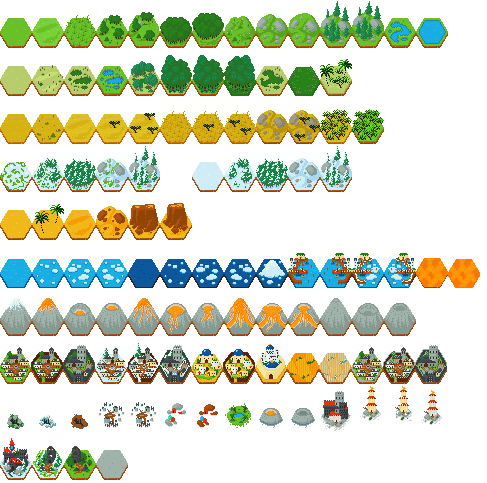
\includegraphics[width=0.6\textwidth]{figures/tileset-borderless.png}
\caption{Terrain sprites collection showing diverse landscape elements including forests, mountains, water bodies, and urban areas designed for seamless hexagonal grid integration and procedural terrain generation.}
\label{fig:tileset_borderless}
\end{figure}

\subsection{Localization}
The initial localization plan focuses on English-only implementation to support the research objectives and target audience. The technical implementation uses a string-based localization system with clear naming conventions for all user-facing text elements. Localization strings are organized by functional categories such as UI elements, tutorial content, mathematical explanations, and error messages. The system is designed to support future expansion to additional languages, particularly for international educational applications. String naming conventions follow a hierarchical structure that clearly identifies the context and purpose of each text element, facilitating future localization efforts and maintenance.

\subsection{Tools}
The development process utilizes several specialized tools to support the game's technical and educational objectives. World creation and layout tools include the TiledProceduralHexTerrainGenerator for terrain generation and custom Unity tools for level design and city-state placement. Object definition tools support the creation and management of game objects with their mathematical properties and visual representations. Mission and quest tools enable the creation of diverse problem instances with varying complexity and educational objectives. Additional tools include data visualization utilities for analyzing player performance and learning outcomes, optimization testing frameworks for validating mathematical solutions, and educational content management systems for organizing tutorial materials and mathematical explanations.

\subsection{Technical Documentation}
The technical implementation addresses several major areas and potential risks. The primary technical challenge involves the real-time integration of mathematical optimization algorithms with game engine performance requirements. The target hardware specifications are designed to ensure accessibility for educational institutions while supporting the computational demands of the ILP solver. The infrastructure includes a modular architecture with clear separation between game logic, mathematical computation, and user interface components. The directory structure follows established conventions for Unity projects with additional organization for mathematical libraries and educational content. Data file formats are designed for efficiency and maintainability, with JSON-based configuration files for level data and mathematical parameters. The server-client architecture is simplified for the educational context, with all computation performed locally to ensure reliability and accessibility. The artificial intelligence and procedural systems include the level generation algorithms, difficulty balancing mechanisms, and adaptive learning systems that adjust to player performance and educational needs. Technical documentation for each major feature includes implementation details, mathematical formulations, and integration guidelines for future development and research applications.

\section{Game Design and Mechanics}

\subsection{Alliance Divider: From ``Links'' to ``Alliances''}
The Alliance Divider game transforms the abstract mathematical problem into an intuitive political strategy game:

\subsubsection{Setting}
\begin{itemize}
  \item Multiple city-states with territories and complex political relationships
  \item Some relationships are friendly, others hostile
  \item City-states may form alliances based on their connections
\end{itemize}

\subsubsection{Player Role}
\begin{itemize}
  \item Royal Strategist analyzing political networks
  \item Discover hidden alliance patterns from relationship dynamics
  \item Make strategic decisions to optimize alliance formation
\end{itemize}

\subsubsection{Goal}
\begin{itemize}
  \item Cut hostile ties while preserving friendly alliances
  \item Form stable alliance clusters
  \item Minimize the total cost of cuts while maintaining valid partitions
\end{itemize}

\subsection{Game Interface and HUD}
The game provides an intuitive interface designed to support both gameplay and educational objectives. The interface includes a level display for current level information and progress tracking, a cut limit display showing remaining cuts available to the player, and a cost display indicating the current total cost of performed cuts. The territory display provides visual representation of alliance clusters, while the hint function offers access to optimal solution hints for educational purposes. Additionally, a revert function allows players to undo their last action, facilitating experimentation and learning through trial and error.

\begin{figure}[h]
\centering
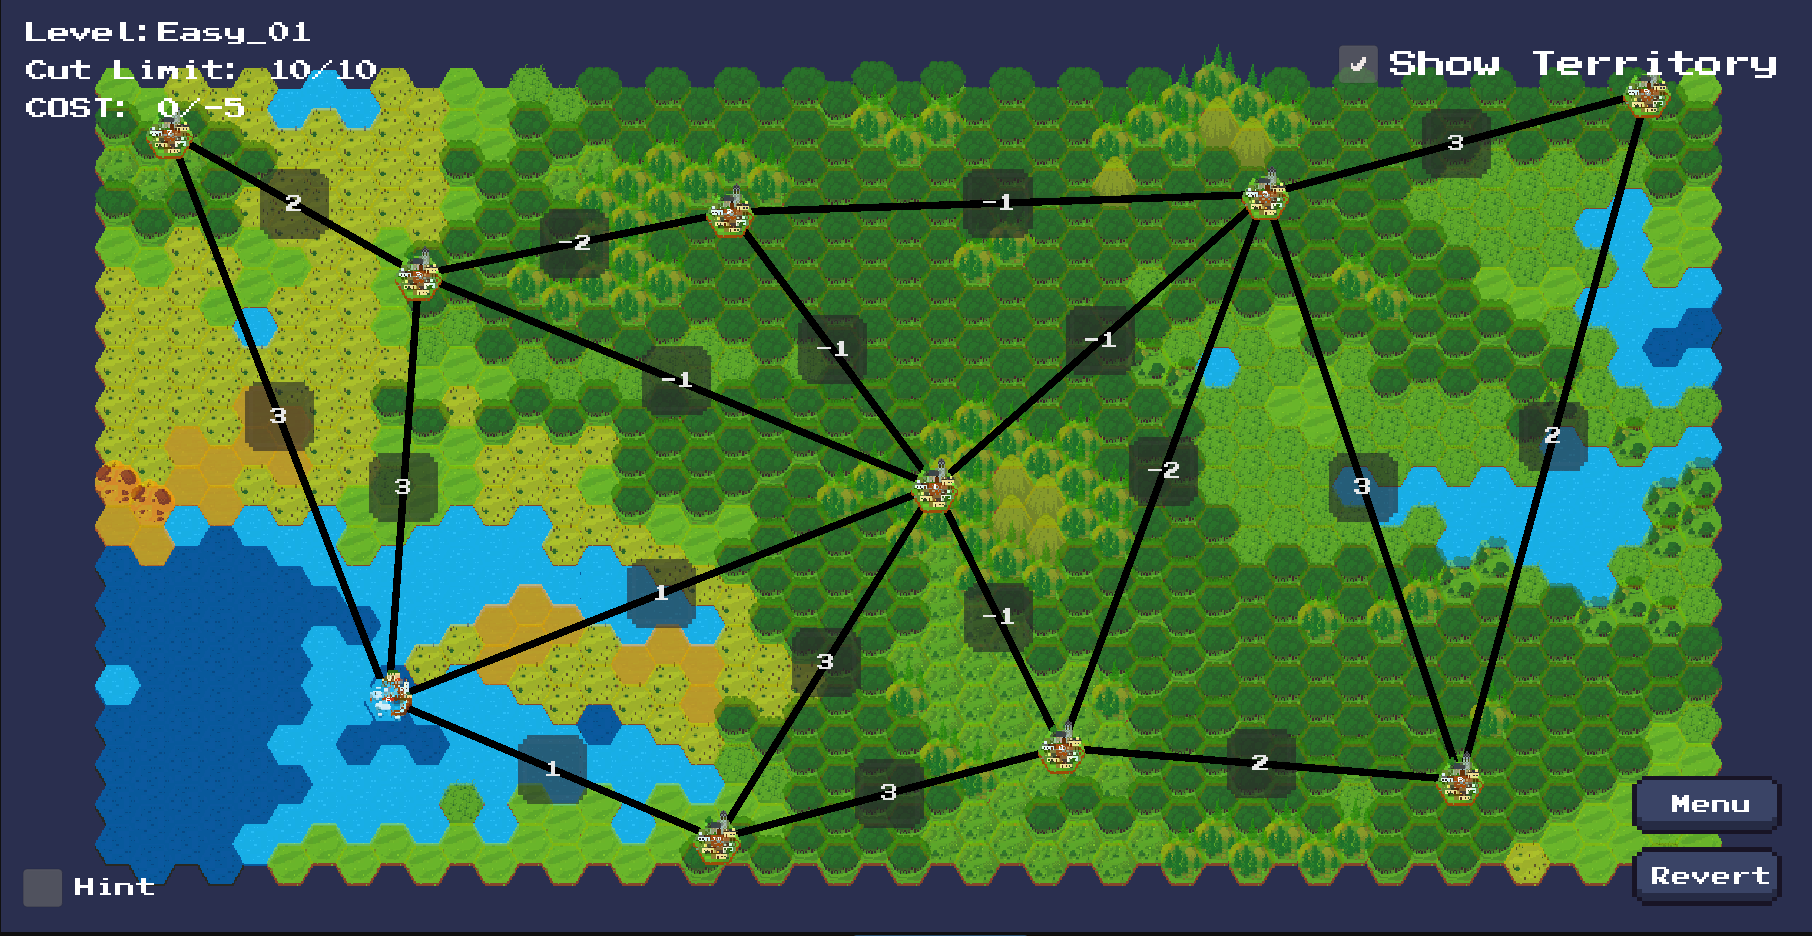
\includegraphics[width=0.8\textwidth]{figures/game_interface.png.png}
\caption{Alliance Divider game interface showing hexagonal terrain, city-states, and UI elements including cost display, level information, and cut limit indicators.}
\label{fig:game_interface}
\end{figure}

\section{Technical Implementation}

The technical implementation of Alliance Divider involves several key components working together to create a seamless educational gaming experience. The project utilizes Unity as the primary game engine, Python for optimization algorithms, and Gurobi as the mathematical solver, creating a cross-language architecture that leverages the strengths of each technology.

\begin{figure}[h]
\centering
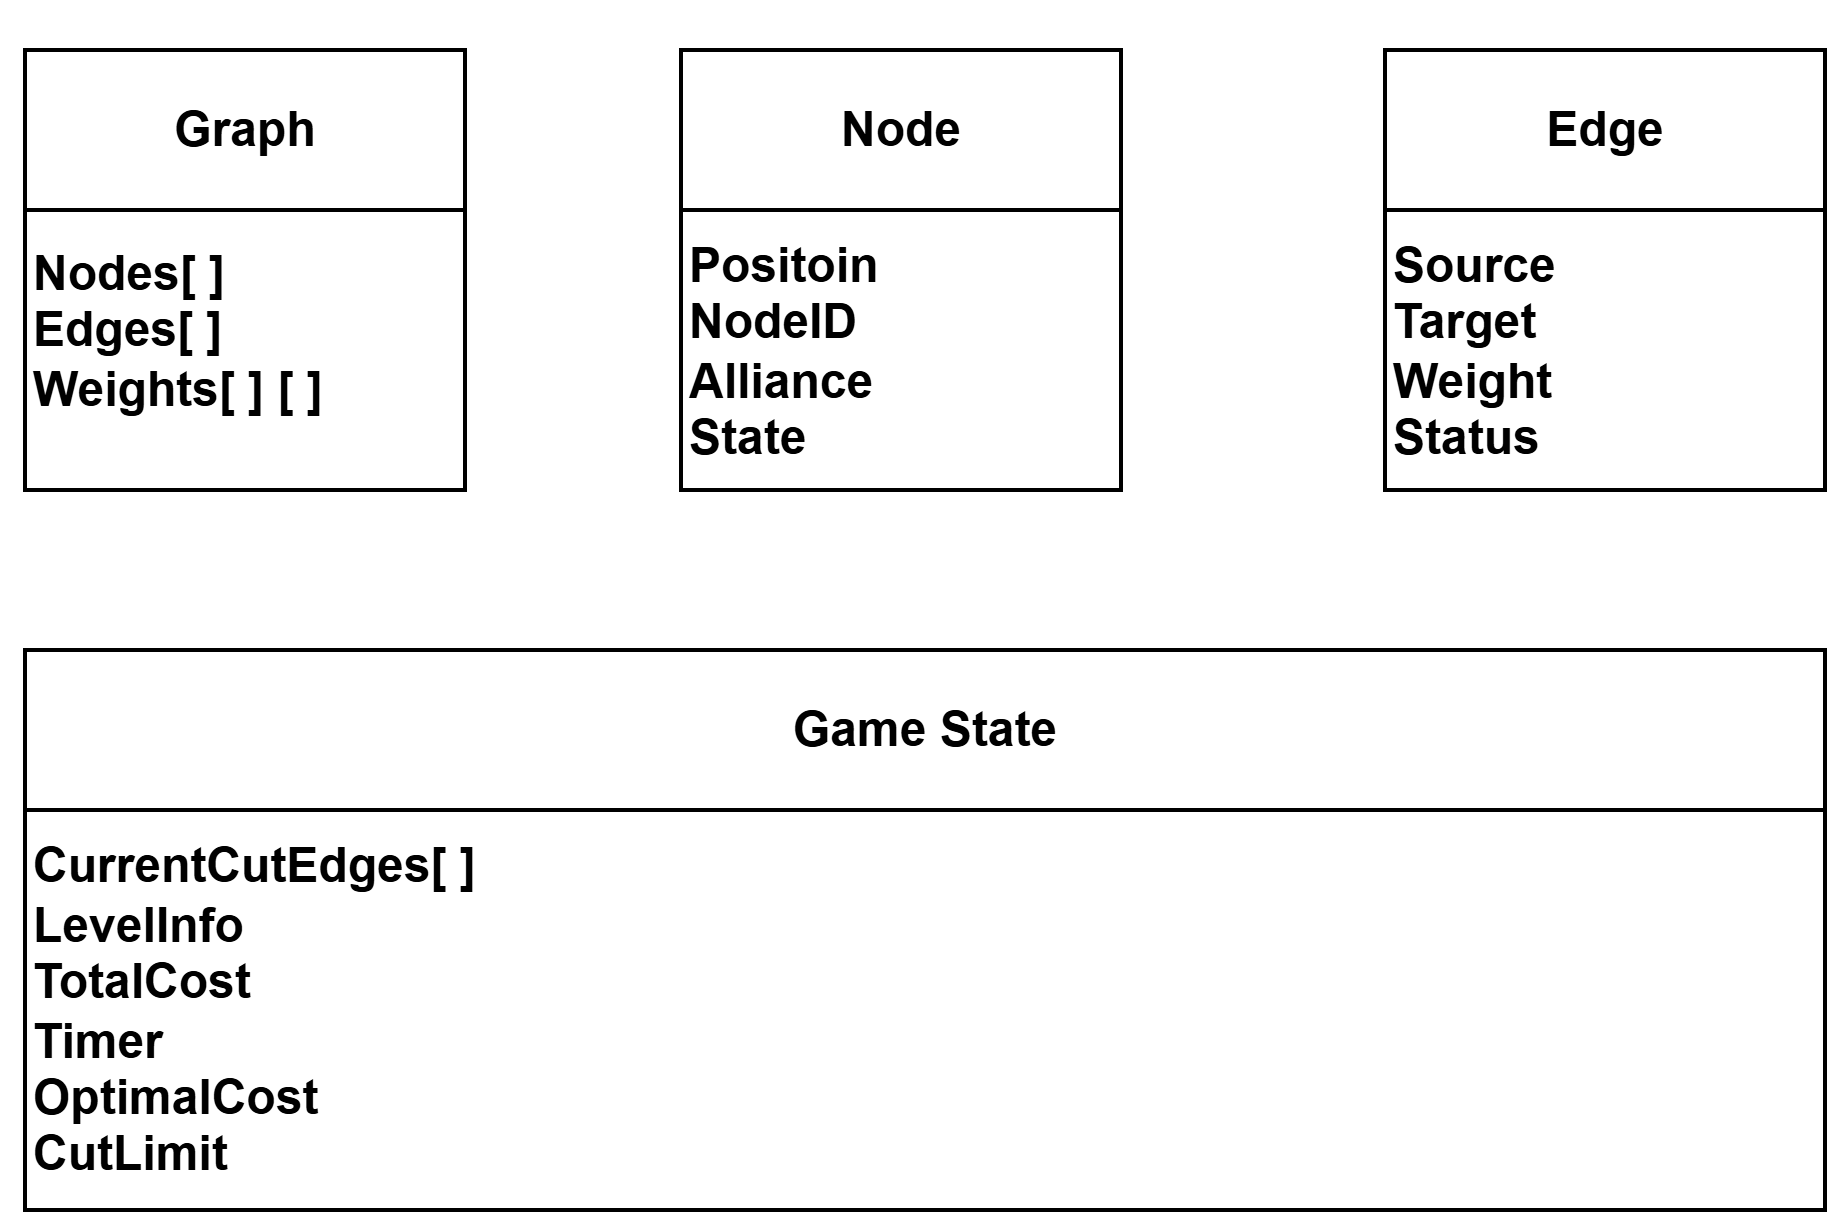
\includegraphics[width=0.7\textwidth]{figures/data_structures.png}
\caption{Core data structures of the Multicut Game showing the Graph, Node, Edge, and Game State components and their relationships.}
\label{fig:data_structures}
\end{figure}

\subsection{Core Data Structures}
The game's technical foundation is built upon a carefully designed set of data structures that efficiently represent the mathematical concepts while supporting real-time gameplay requirements. As illustrated in Figure~\ref{fig:data_structures}, the core data structures form a hierarchical system that bridges the gap between mathematical graph theory and interactive game mechanics.

\paragraph{Graph Structure}
The central data structure is the Graph class, which maintains the complete mathematical representation of the game state. This structure contains a collection of nodes (city-states) and edges (relationships), with each element possessing both mathematical properties and visual representation data. The graph structure supports efficient traversal algorithms for alliance detection and territory coloring, while maintaining the mathematical integrity required for the Multicut Problem solution.

\paragraph{Node Representation}
Each node in the graph represents a city-state with comprehensive attributes including position coordinates (both hexagonal axial and Unity world coordinates), alliance membership, visual state, and relationship weights with neighboring nodes. The node structure supports dynamic updates during gameplay, allowing for real-time visual feedback when alliances change due to edge cuts. The coordinate system conversion between hexagonal axial coordinates (q,r) and Unity world coordinates (x,y) is handled efficiently through optimized mathematical transformations.

\paragraph{Edge Management}
Edges represent the relationships between city-states, with each edge containing weight values (positive for friendly relationships, negative for hostile ones), connection status, visual representation data, and mathematical properties required for the Multicut algorithm. The edge structure supports efficient weight calculations, cut operations, and visual updates, ensuring that the mathematical operations remain synchronized with the visual representation throughout gameplay.

\paragraph{Game State Management}
The Game State structure maintains the overall game state including current level information, player progress, cut history, and optimization results. This structure serves as the central coordinator between the mathematical solver, visual representation, and user interface systems. The game state supports save/load operations, level progression tracking, and performance optimization through intelligent caching mechanisms.

\subsection{Unity Game Engine Integration}
Unity was chosen as the primary development platform due to its widespread adoption, active community support, rich resource ecosystem, and cross-platform development capabilities. The engine provides essential features including Tilemap system for hexagonal terrain generation, Sprite system for city-state visualization, Raycast system for collision detection, LineRenderer for edge visualization, and comprehensive UI tools for interface development. Unity's prefab system enables component reusability, while its serialization capabilities facilitate debugging and data persistence.

The integration of Unity with external mathematical solvers presented significant technical challenges. Initial attempts to integrate Gurobi's C\# API directly with Unity encountered DLL loading issues, necessitating a shift to Python script execution. This challenge led to the development of a robust cross-language communication system using JSON file exchange, which proved more reliable than direct API integration.

\subsection{System Architecture Overview}
The overall technical architecture consists of seven distinct layers working in harmony:

\textbf{Game Engine Layer (Unity):} The core rendering platform utilizing Unity 2D engine, Tilemap system for terrain management, 2D physics system for collision detection, and URP (Universal Render Pipeline) for rendering. This layer handles scene management, object lifecycle, user input processing, real-time rendering, UI systems, and coroutine management for asynchronous operations.

\textbf{Terrain Generation Layer:} A sophisticated hexagonal terrain system featuring custom coordinate systems supporting axial and world coordinate conversion, noise generators for height and moisture maps, biome mapping systems, and river generation networks. The tilemap system integrates with Unity Tilemap, converting hexagonal terrain to tile grids with comprehensive coordinate transformation capabilities.

\textbf{Graph Theory Algorithm Layer:} Implements grid generation using Delaunay triangulation with refinement algorithms, Poisson disk distribution for node placement, and multicut algorithms with cycle inequality constraints. The weight system design uses positive weights for important edges and negative weights for cuttable edges.

\textbf{External Solver Layer (Python-Gurobi):} A decoupled architecture where Unity communicates with Python scripts through JSON files, with Python calling Gurobi solver for NP-hard problem resolution. The data flow involves Unity serializing graph structures to input.json, Python modeling the multicut problem, Gurobi solving for optimal cuts, and results written to output.json for Unity consumption.

\textbf{Game Logic Layer:} Manages level systems with difficulty grading (Easy, Medium, Hard), level generators with parameter adjustment, victory condition detection, cutting line systems, edge weight visualization, and hint systems for optimal cut highlighting.

\textbf{Data Management Layer:} Handles game state management, edge weight caching, territory highlighting, PlayerPrefs for user settings and progress, scene selection, and terrain data export/import functionality.

\textbf{Visualization Layer:} Provides territory display with background calculation systems, cluster merging based on cut edges, highlighting systems for different territories, and comprehensive debugging tools including weight calculators and terrain traversal detection visualization.

\begin{figure}[h]
\centering
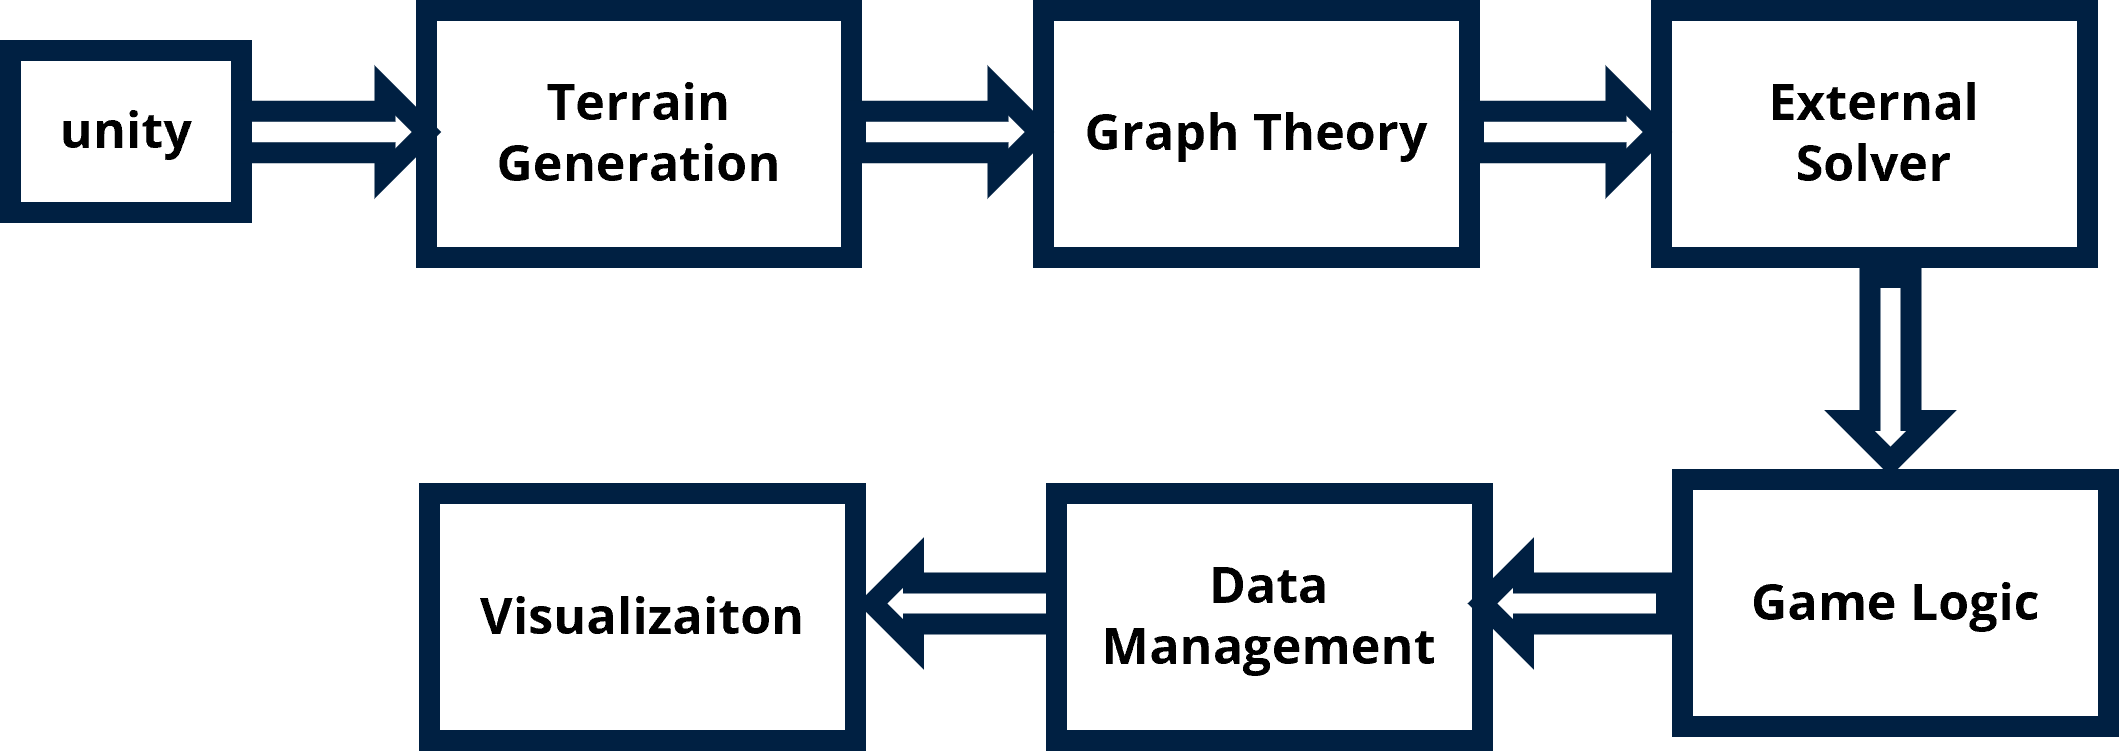
\includegraphics[width=0.8\textwidth]{figures/system_architecture.png}
\caption{System architecture overview showing the seven-layer structure from Game Engine Layer to Visualization Layer, demonstrating the data flow and component interactions.}
\label{fig:system_architecture}
\end{figure}

\subsection{Game Scene Generation and Optimization}
The game scene generation system employs sophisticated algorithms to create visually appealing and mathematically sound game environments. This system ensures that each generated level provides both educational value and engaging gameplay while maintaining optimal performance across different hardware configurations.

\subsubsection{City-State Position Generation with Poisson Disk Sampling}
The city-state positioning system utilizes Poisson Disk Sampling to ensure optimal spatial distribution of nodes across the hexagonal terrain. This algorithm guarantees that no two city-states are placed too close to each other, preventing visual clutter and ensuring clear representation of the graph structure.

\textbf{Algorithm Implementation:}
The Poisson Disk Sampling algorithm operates by maintaining a minimum distance constraint between all placed points. The implementation uses a grid-based approach to efficiently check distance constraints, ensuring that each new city-state placement maintains the required minimum separation from all existing city-states.



The algorithm provides several key features including minimum distance constraints for visual clarity, random distribution for natural layouts, performance optimization through spatial partitioning, and adaptive density adjustment based on terrain complexity and difficulty level. These features ensure clear separation between city-states, create organic-looking political landscapes, efficiently handle varying numbers of city-states, and provide clear visual representation that aids in understanding graph structures.

\subsubsection{Connection Generation via Delaunay Triangulation}
The connection generation system employs Delaunay Triangulation to create optimal networks of relationships between city-states. This algorithm ensures that the generated graph structure is mathematically sound and provides a natural foundation for the multicut problem.

\textbf{Mathematical Foundation:}
Delaunay Triangulation creates a triangulation where no point lies inside the circumcircle of any triangle. This property ensures that the resulting triangulation maximizes the minimum angle of all triangles, creating a well-structured and visually appealing network.

\textbf{Algorithm Process:}
\begin{enumerate}
  \item \textbf{Point Set Preparation}: Organize city-state positions into a valid input set
  \item \textbf{Initial Triangulation}: Create a super-triangle that contains all points
  \item \textbf{Incremental Insertion}: Add points one by one, maintaining Delaunay properties
  \item \textbf{Edge Refinement}: Optimize triangle quality and remove thin triangles
  \item \textbf{Final Network}: Extract the dual graph to create the connection network
\end{enumerate}



The algorithm provides optimization features including angle optimization to maximize minimum angles, edge quality control for visually clear connections, performance scaling for varying numbers of city-states, and maintenance of desirable graph-theoretic properties. These features create realistic political relationship networks, ensure mathematical rigor suitable for multicut algorithms, produce aesthetically pleasing connection patterns, and provide clear visual representation of graph theory concepts.

\subsubsection{Automatic Centering and Scaling}
The automatic centering and scaling system ensures that generated game scenes are optimally positioned and sized for different display configurations. This system provides consistent gameplay experience across various screen resolutions and aspect ratios.

\textbf{Centering Algorithm:}
The system calculates the bounding box of all placed city-states and their connections, then centers this bounding box within the available screen space. This ensures that the game scene is always optimally positioned regardless of the number or distribution of city-states.

The scaling implementation includes dynamic scaling to automatically adjust scene size, aspect ratio handling to maintain proper proportions, margin management to ensure adequate spacing, and zoom level optimization for optimal visibility. Performance considerations include real-time calculation algorithms, memory optimization for minimal overhead, cross-platform compatibility for consistent behavior, and smooth user experience transitions. These features provide consistent gameplay experience across different devices, ensure accessibility on various screen sizes, deliver professional visual presentation, and enhance educational effectiveness through optimal viewing conditions.

\subsection{Third-Party TileMap Generator Integration}
The game incorporates advanced tilemap generation systems to create diverse and visually appealing game environments, enhancing the overall user experience.

\subsubsection{TiledProceduralHexTerrainGenerator}
The game utilizes the TiledProceduralHexTerrainGenerator\footnote{Available at: \url{https://github.com/HextoryWorld/TiledProceduralHexTerrainGenerator}} for sophisticated terrain generation.

\textbf{Terrain Generation Steps:}
\begin{enumerate}
  \item Generate a random heightmap as the base terrain foundation
  \item Overlay multiple layers of details to create natural terrain variations
  \item Classify terrain types based on height and environmental factors
  \item Add humidity variations to create diverse ecosystems
\end{enumerate}

\textbf{Integration Steps:}
\begin{enumerate}
  \item \textbf{Calculate World Coordinates}: Convert tilemap coordinates (q,r) to Unity world coordinates (x,y)
    \begin{align}
      X &= \text{hexSize} \times \frac{3}{2} \times q \\
      Y &= \text{hexSize} \times \sqrt{3} \times \left(\frac{q}{2} + r\right)
    \end{align}
    where $X$ and $Y$ are Unity world coordinates, $q$ and $r$ are hexagonal axial coordinates, and $\text{hexSize}$ is the size parameter of the hexagonal grid.
  \item \textbf{Handle Coordinate Offset}: Adjust for Unity's origin at screen center (0,0)
  \item \textbf{Invert Y-axis}: Convert between different coordinate system conventions
\end{enumerate}

\begin{figure}[h]
\centering
\begin{subfigure}[b]{0.32\textwidth}
    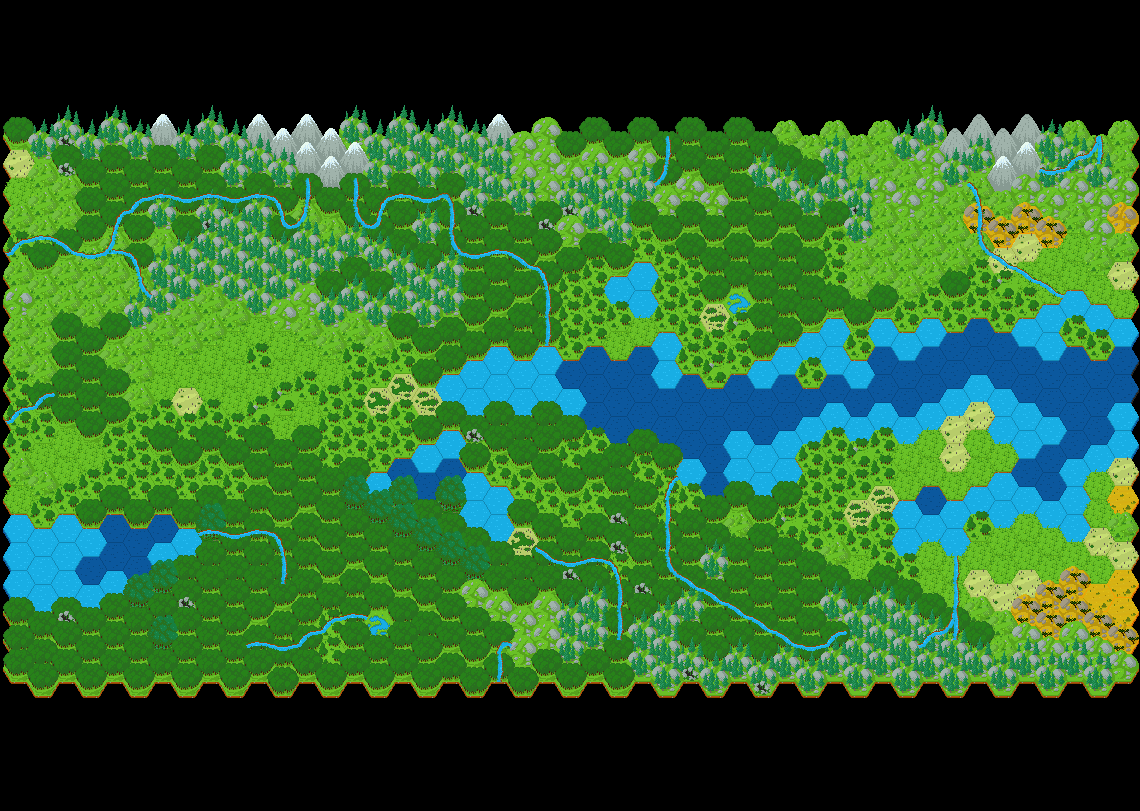
\includegraphics[width=\textwidth]{figures/hexGrid1.png}
    \caption{Random terrain generation example 1}
    \label{fig:terrain_1}
\end{subfigure}
\hfill
\begin{subfigure}[b]{0.32\textwidth}
    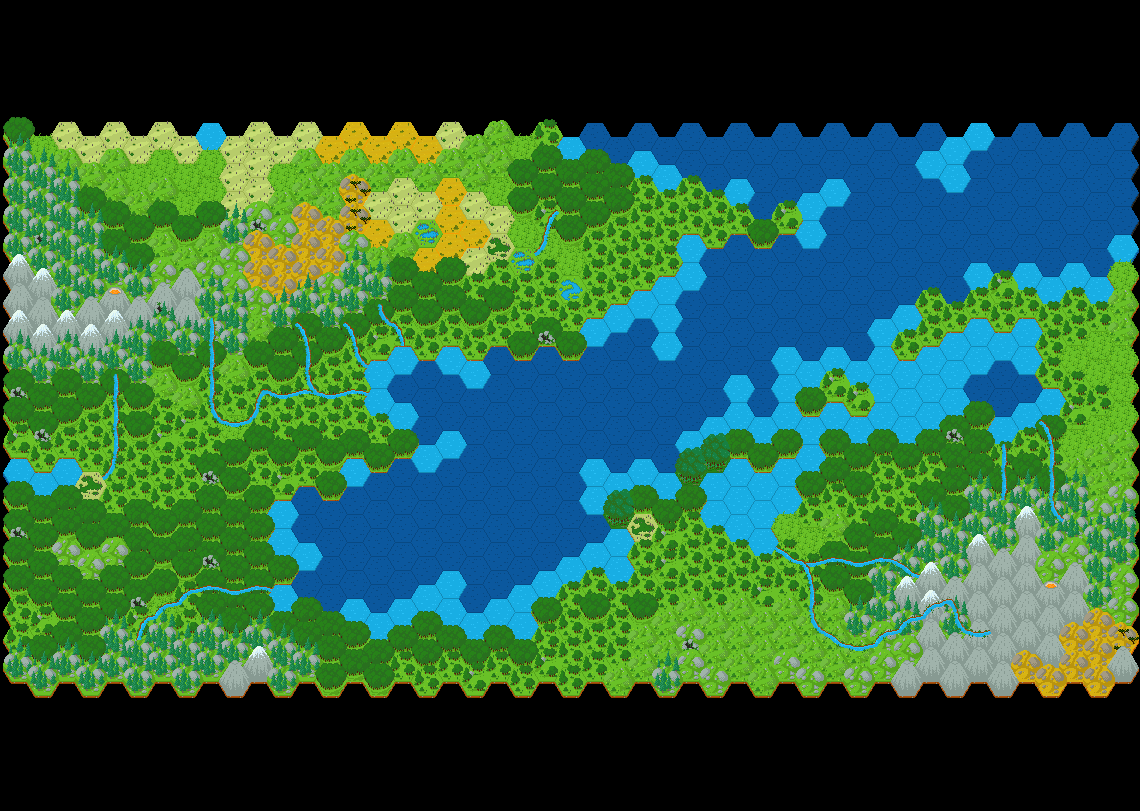
\includegraphics[width=\textwidth]{figures/hexGrid2.png}
    \caption{Random terrain generation example 2}
    \label{fig:terrain_2}
\end{subfigure}
\hfill
\begin{subfigure}[b]{0.32\textwidth}
    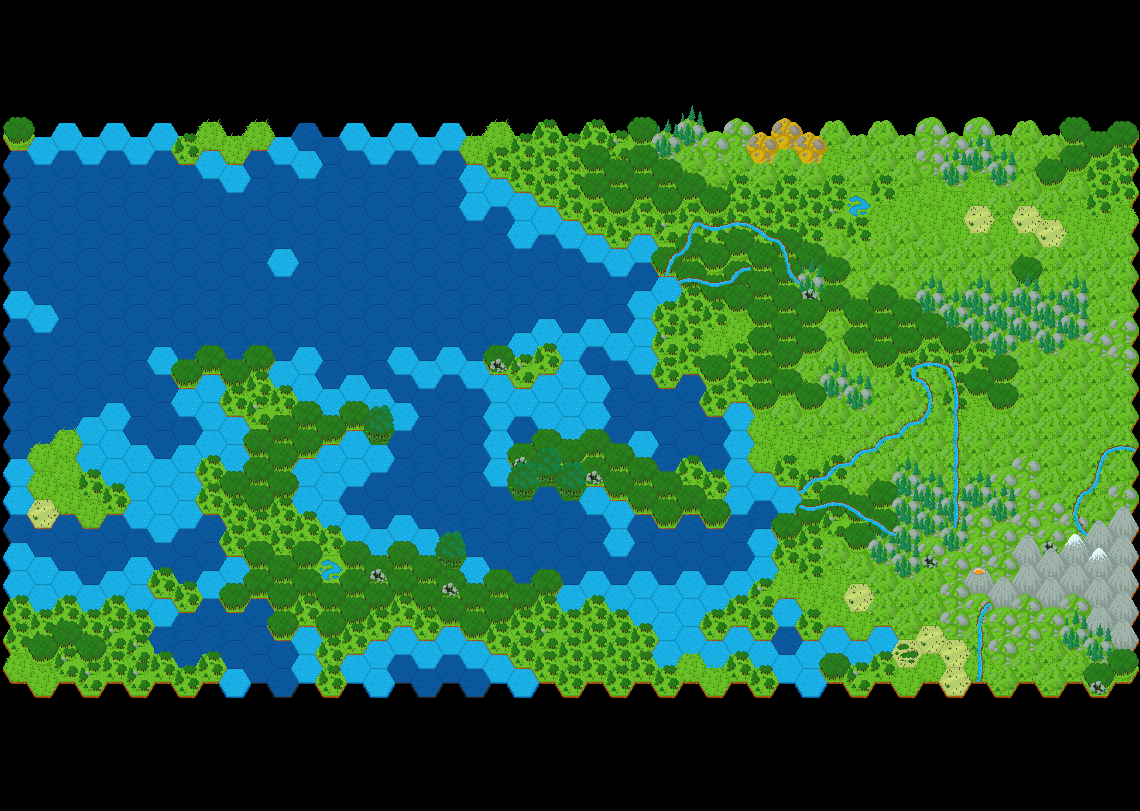
\includegraphics[width=\textwidth]{figures/hexGrid3.png}
    \caption{Random terrain generation example 3}
    \label{fig:terrain_3}
\end{subfigure}

\vspace{0.5cm}

\begin{subfigure}[b]{0.32\textwidth}
    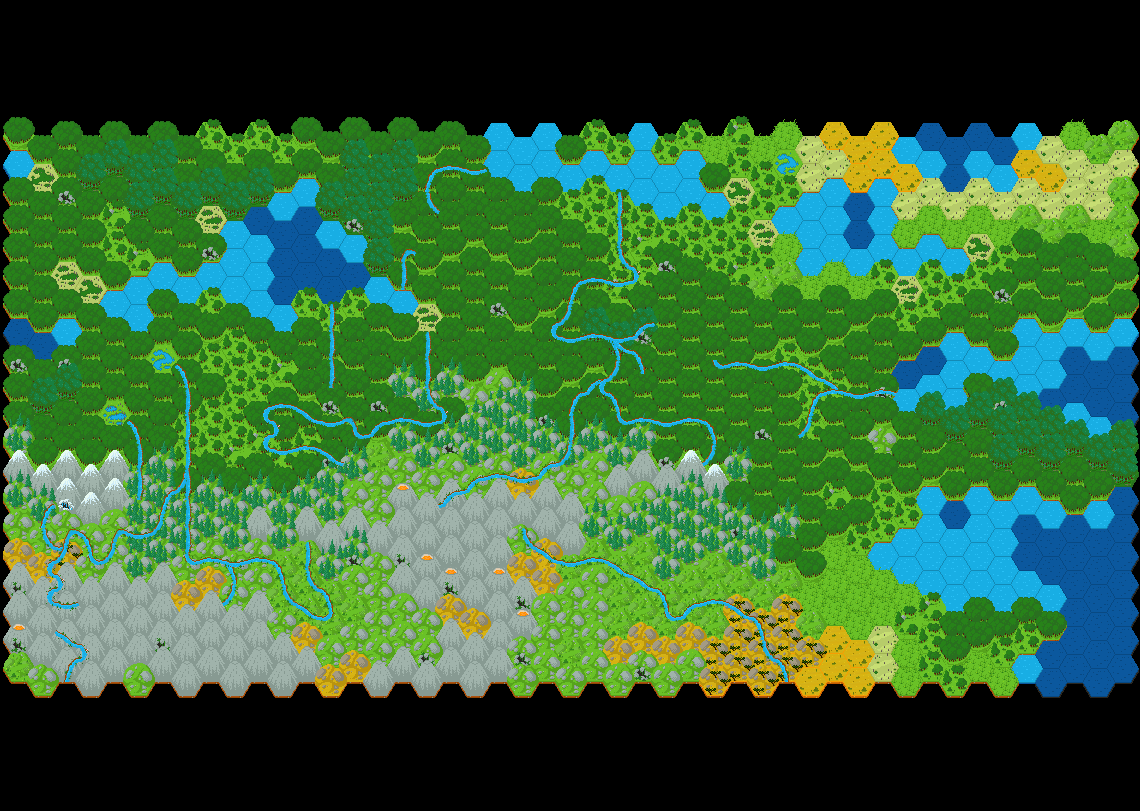
\includegraphics[width=\textwidth]{figures/hexGrid4.png}
    \caption{Random terrain generation example 4}
    \label{fig:terrain_4}
\end{subfigure}
\hfill
\begin{subfigure}[b]{0.32\textwidth}
    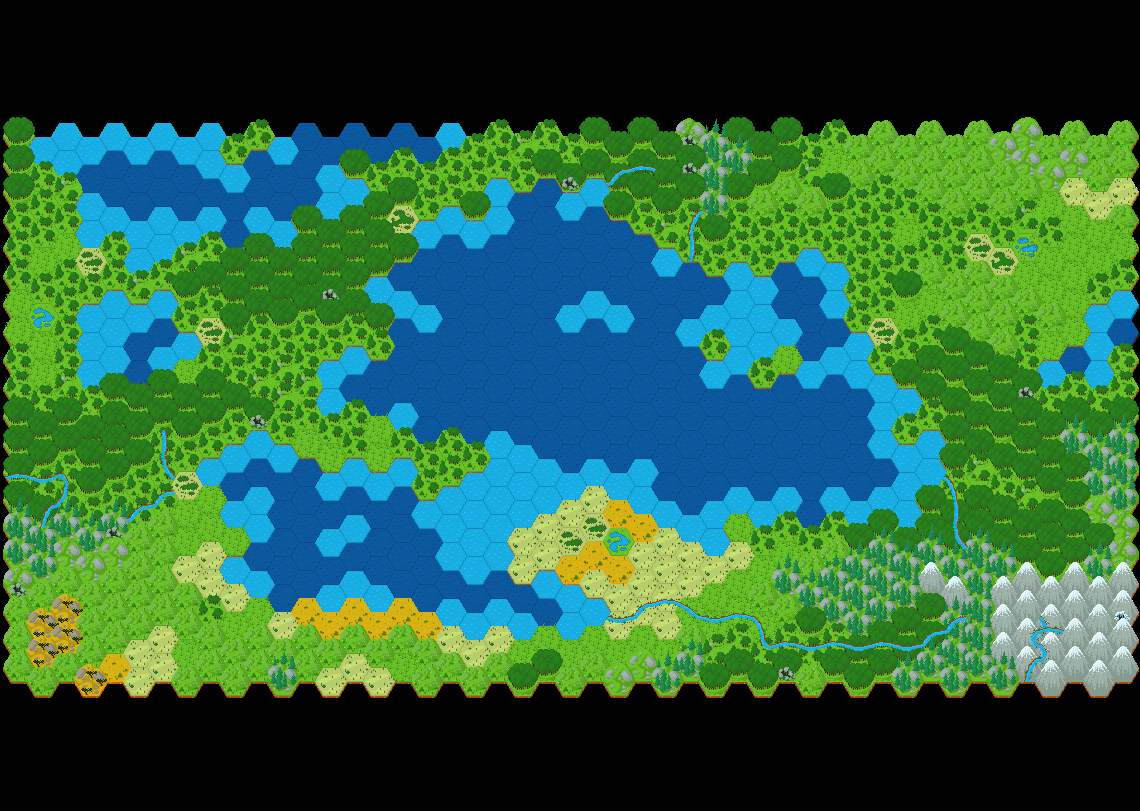
\includegraphics[width=\textwidth]{figures/hexGrid5.png}
    \caption{Random terrain generation example 5}
    \label{fig:terrain_5}
\end{subfigure}
\hfill
\begin{subfigure}[b]{0.32\textwidth}
    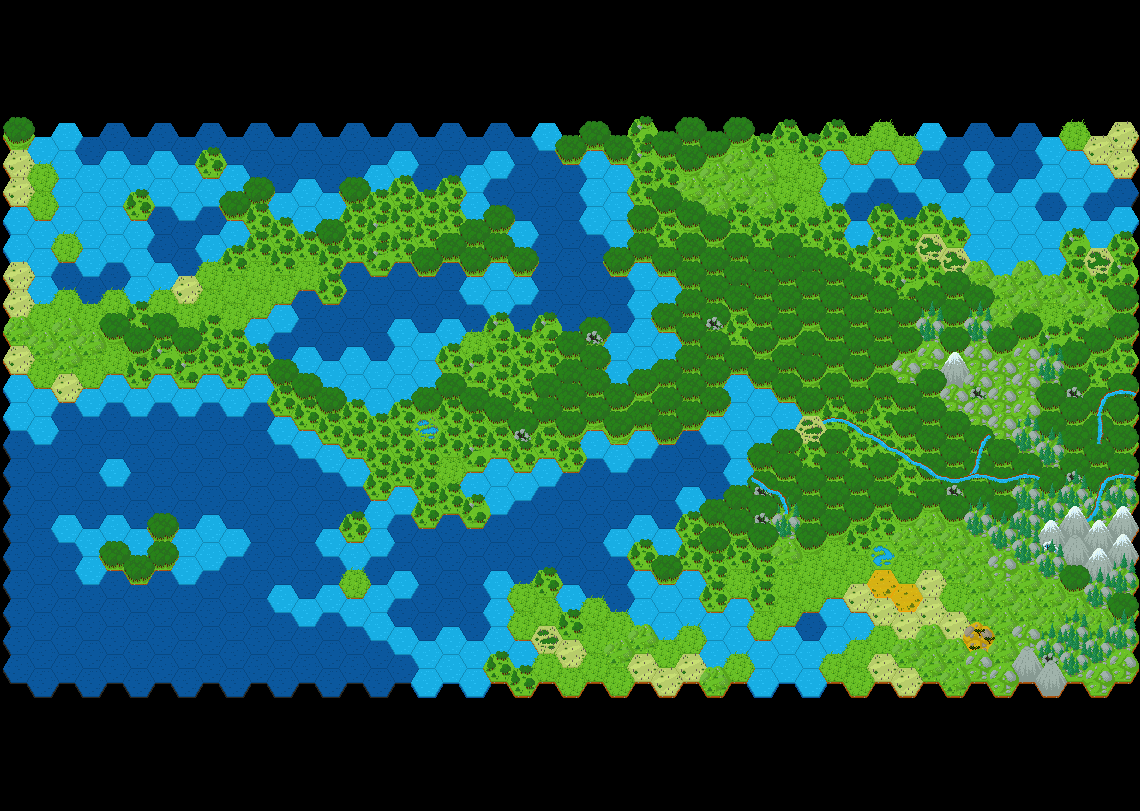
\includegraphics[width=\textwidth]{figures/hexGrid6.png}
    \caption{Random terrain generation example 6}
    \label{fig:terrain_6}
\end{subfigure}
\caption{Six examples of procedurally generated terrain maps using the same parameters, demonstrating the random yet artistically pleasing visual effects of the TiledProceduralHexTerrainGenerator.}
\label{fig:terrain_generation_examples}
\end{figure}


\subsubsection{Coordinate System Conversion}
The project implements a sophisticated coordinate system conversion mechanism to handle multiple coordinate systems simultaneously:

\textbf{Hexagonal Coordinate System Conversion:} The system uses custom hexagonal coordinate systems with axial coordinates (q,r) and world coordinates (x,y,z) conversion. Axial coordinates use q for columns and r for rows, converted to Unity world coordinates through mathematical formulas. The conversion considers hexagonal orientation (flat or pointy) using different transformation matrices.

\textbf{Tilemap Coordinate System Conversion:} TerrainManager implements hexagonal coordinate to Unity Tilemap coordinate conversion. This process converts axial coordinates to tile grid coordinates with centering to position terrain around the origin. The conversion requires X and Y coordinate swapping to match expected layouts.

\textbf{World Coordinate and Tilemap Coordinate Conversion:} Unity's Tilemap system provides WorldToCell and CellToWorld methods for coordinate conversion, used extensively for terrain detection and edge traversal detection. These methods ensure accurate coordinate representation across different systems.

\textbf{Coordinate System Unification:} The project addresses coordinate system inconsistencies through unified (X,Y,Z) format usage, ensuring all systems use consistent coordinate representation. Reflection technology is employed to access TerrainManager mapping tables, avoiding direct type references that could cause coordinate system conflicts.

\textbf{Performance Optimization:} Coordinate conversion performance is optimized through result caching and reduced redundant calculations, particularly in terrain weight computation to avoid repeated coordinate conversions.

\begin{figure}[h]
\centering
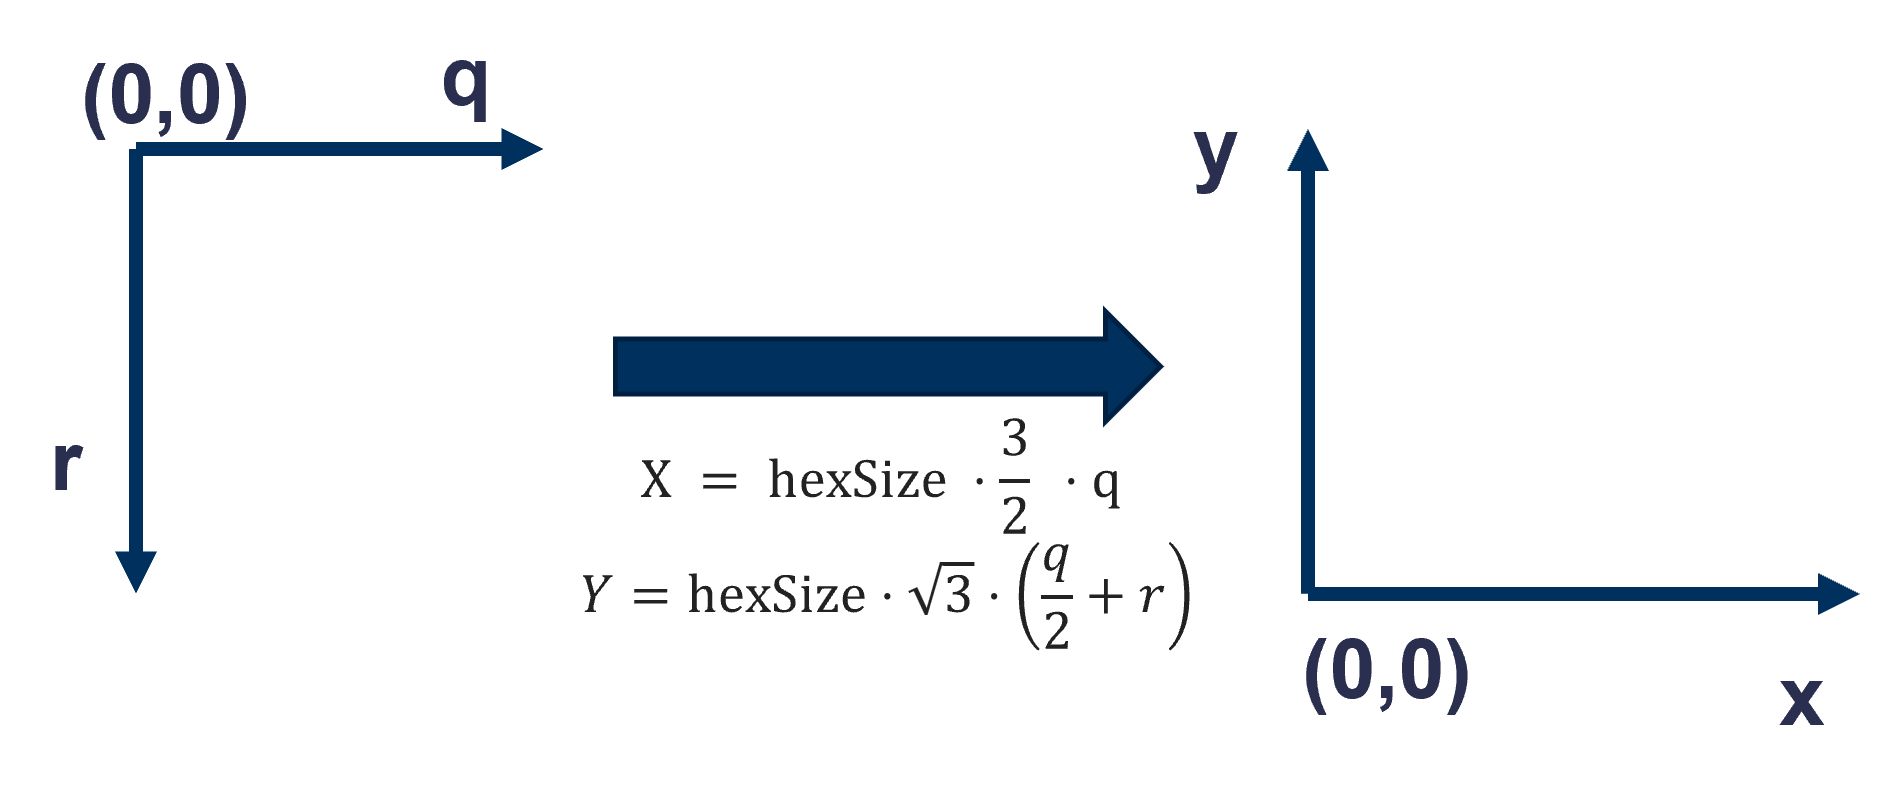
\includegraphics[width=0.6\textwidth]{figures/coordinate_system.png}
\caption{Coordinate system conversion diagram showing the transformation from hexagonal axial coordinates (q,r) to Unity world coordinates (x,y) and the mathematical relationships between different coordinate systems.}
\label{fig:coordinate_system}
\end{figure}

\subsection{Solving the Multicut Problem: ILP + Gurobi}
The core optimization engine utilizes Integer Linear Programming with Gurobi solver to address the NP-hard nature of the multicut problem.

\textbf{Challenge:} Multi-cut is NP-hard—exact solutions are computationally expensive.

\begin{table}[h]
\centering
\caption{Comparison of Solution Approaches for Multicut Problem}
\begin{tabular}{p{3cm}p{4cm}p{5cm}}
\toprule
\textbf{Method} & \textbf{Performance} & \textbf{Solution Quality} \\
\midrule
Heuristic & Fast & Cannot guarantee optimality \\
\midrule
Approximation & Moderate & Poor results \\
\midrule
Brute-force & Infeasible & Optimal but impractical \\
\midrule
ILP & Fast & Theoretically optimal \\
\bottomrule
\end{tabular}
\end{table}

The Gurobi ILP approach provides the optimal balance between computational efficiency and solution quality, making it suitable for real-time game applications while maintaining mathematical rigor.

\subsection{System Integration: Unity to Python Cross-Language Integration}

\subsubsection{Architecture Overview}
The system implements a robust cross-language integration between Unity (C\#) and Python for optimization tasks. The architecture utilizes a C\# Process Class to launch Python processes for optimization tasks, with JSON files serving as the exchange medium for data transfer between Unity and Python. The input data consists of graph structure and edge weight information, while the output data includes cut edges and optimal cost calculations, enabling seamless communication between the game engine and optimization solver.

\subsubsection{Unity-Python Integration Details}
The Unity-Python integration follows a comprehensive four-step workflow:

\textbf{Unity End Data Preparation:} The system serializes graph structures (Cells) and edge weights into JSON format, writing to input.json file containing node information and edge weight data. This process ensures data compatibility between Unity's C\# environment and Python's mathematical processing capabilities.

\textbf{Python Script Invocation:} Unity launches the optimization solver script through system process calls. The system process starts the Python interpreter to execute optimization tasks.

\textbf{Python End Processing:} The Python script reads input.json file, uses Gurobi to model the multicut problem, solves for optimal cutting schemes, and writes results to output.json for Unity consumption.

\textbf{Unity End Result Reading:} Unity monitors output.json file changes, parses optimal cut edge lists and cost values, and updates UI displays and cut edge highlighting accordingly.

\textbf{Data Format Specifications:} Input data includes node information (position, number), edge information (connection relationships, weight values), and graph structure (adjacency matrix or edge list). Output data contains cut edge lists (edge numbers to be cut), optimal cost values (algorithm-calculated optimal solutions), and status information (solution success indicators).

\subsubsection{Integration Flow}
The integration follows a specific workflow:

\begin{enumerate}
  \item \textbf{Unity (C\#)} provides data (nodes, edges) to the optimization system
  \item \textbf{C\# Process} creates and manages the Python execution environment
  \item \textbf{Python} builds the ILP model based on the input graph data
  \item \textbf{Gurobi Solver} finds the optimal solution through industrial-grade optimization
  \item \textbf{Solution Return}: The optimal solution (cut edges, optimal cost) is returned to Unity for game state updates
\end{enumerate}

\subsubsection{Benefits of Cross-Language Integration}
The cross-language integration approach offers several significant advantages. Unity provides robust game engine capabilities and user interface \cite{unity2023}, while Python offers extensive mathematical and optimization libraries that are essential for implementing complex algorithms. This modular architecture effectively separates game logic from optimization algorithms, enabling independent development and maintenance of each component while ensuring optimal performance and maintainability.

\begin{figure}[h]
\centering
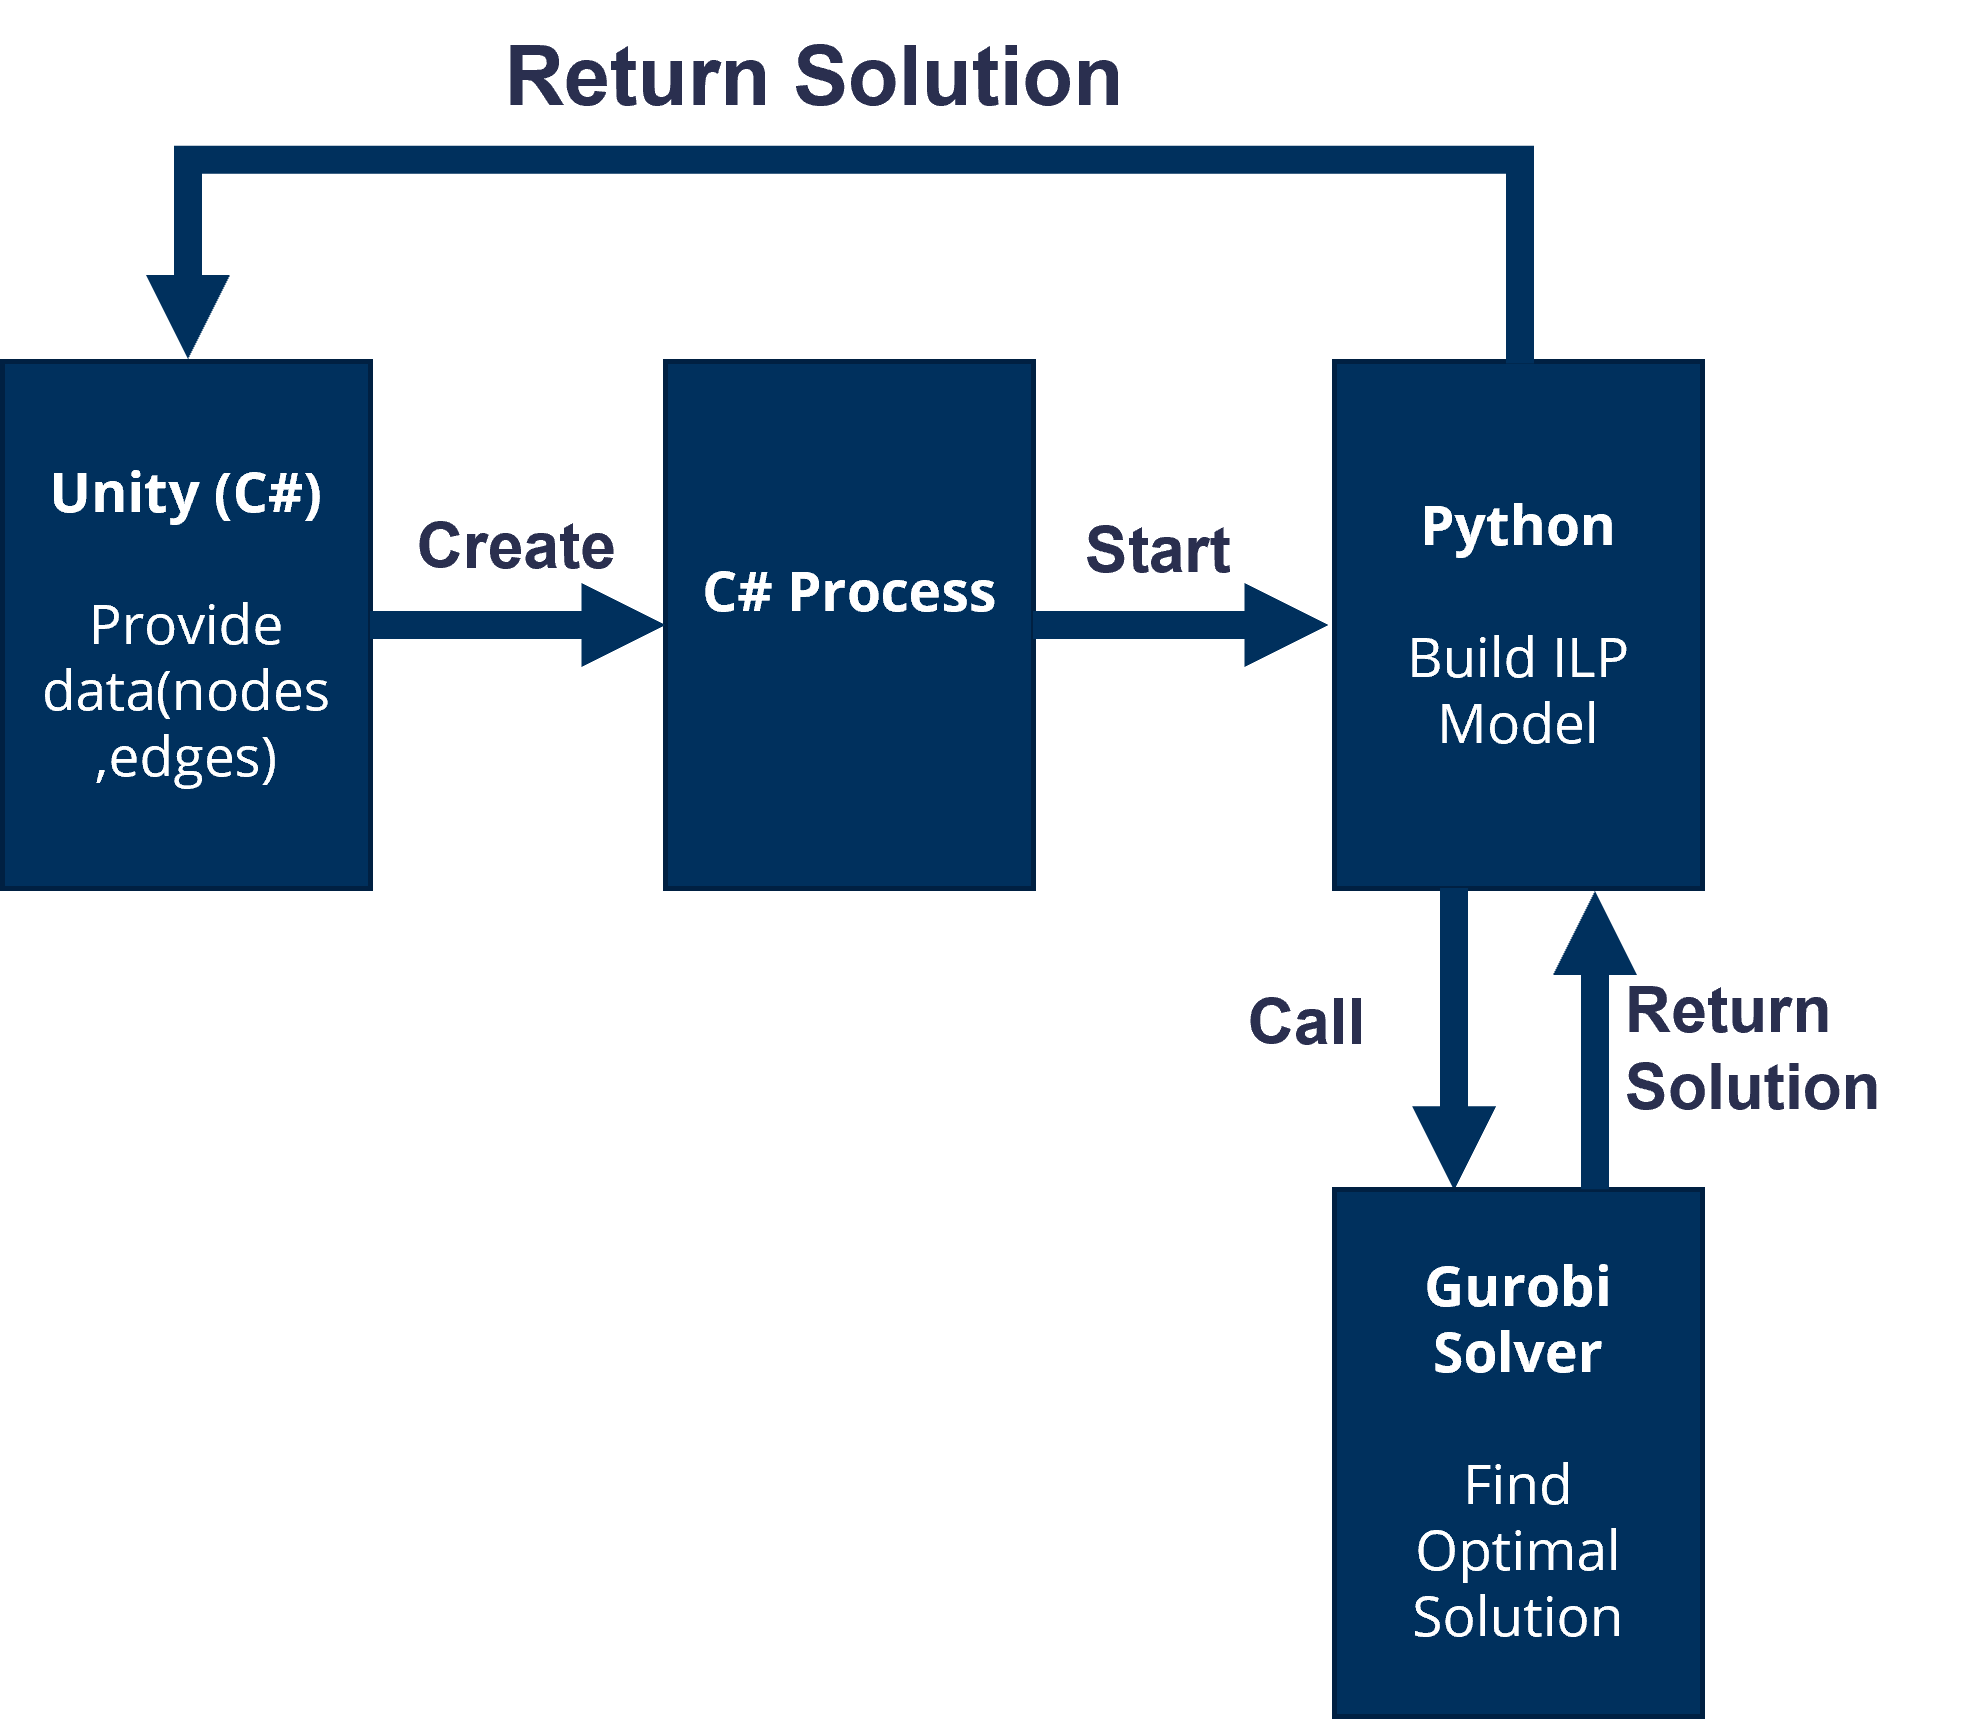
\includegraphics[width=0.8\textwidth]{figures/unity_python_integration.png}
\caption{Unity-Python integration workflow showing the data flow from Unity through JSON files to Python and Gurobi solver, and back to Unity for game state updates.}
\label{fig:unity_python_integration}
\end{figure}

\section{Gamification Design}

\subsection{Core Game Mechanics}
The game's core mechanics are based on the Multicut Problem, where players assume the role of medieval city-state strategists analyzing complex political relationships. The game features multiple city-states (Cells) connected by a complex relationship network (Edges), where positive weights represent ally relationships and negative weights represent hostile relationships. Players must cut edges to minimize hostile relationships while preserving ally relationships, ultimately identifying stable alliance groups. The game uses standard multicut algorithms without limiting the number of connected components, ensuring algorithmic correctness through lazy constraints.

\subsection{Player Interaction System}
Player interaction is primarily mouse-based, with right-click and hold functionality for drawing cutting lines that sever edges when rules permit. Players can reconnect severed edges, and the game provides a Hint button (Toggle form) that highlights optimal cutting edges when activated. The UI interface displays current cost, optimal cost, cut limit count, timer, and other essential information. Players can also use the territory Toggle to view color highlighting of different connected components.

\subsection{Cutting Mechanism Implementation}
The cutting mechanism is implemented through the eraseline system. When players hold right-click to draw cutting lines, the system detects edges traversed by the line and removes them from the graph if they are not in a locked state. The system monitors connected component changes and checks initial edges for reconnection when two isolated connected components are linked by a line. Cut edges are recorded in the playerCutEdges collection for current cost calculation.

\subsection{Victory Condition System}
Victory conditions are based on cost comparison. The system continuously calculates current cost (sum of weights of player-cut edges) and optimal cost (optimal solution calculated by Python algorithm). Victory is achieved when currentCost equals optimalCost, indicating the player has reached the optimal solution. Upon victory, the system displays a victory panel, pauses game time, and provides a continue button to proceed to the next level. Victory detection is performed in real-time through continuous monitoring.

\subsection{Difficulty System Design}
The game implements a progressive three-tier difficulty system with distinct parameters for each level:

\textbf{Easy Mode:} Features cut limit restrictions only, with 8 nodes, moderate average degree, and relaxed time constraints. This mode focuses on teaching basic concepts without time pressure.

\textbf{Medium Mode:} Combines cut limit restrictions with timer functionality, featuring 10 nodes, moderate time constraints, and limited cut quotas. This mode introduces time management challenges.

\textbf{Hard Mode:} Implements cut limit restrictions, timer functionality, and penalty edge mechanics, with 12 nodes, tight time constraints, and penalty edges that increase the cost when cut. This mode provides maximum challenge with multiple constraint layers.

The difficulty adjustment is automated through difficulty setting methods that progressively adjust parameters as levels advance. The complexity increases from Easy to Hard mode, providing appropriate challenge scaling for different skill levels.

\begin{table}[h]
\centering
\caption{Comparison of difficulty levels and their parameters}
\begin{tabular}{lcccc}
\toprule
\textbf{Difficulty} & \textbf{Nodes} & \textbf{Time Limit} & \textbf{Cut Limit} & \textbf{Special Features} \\
\midrule
Easy & 8 & No & Yes & Basic concepts only \\
Medium & 10 & Yes & Yes & Time management \\
Hard & 12 & Yes & Yes & Penalty edges \\
\bottomrule
\end{tabular}
\label{tab:difficulty_comparison}
\end{table}

\subsection{Level Generation System}
The level generation system implements a comprehensive pipeline that transforms spatial point distribution into fully playable game levels. As illustrated in Figure~\ref{fig:level_generation}, the system follows a structured approach from initial generation through refinement to final level output.

\paragraph{Initial Generation Phase}
The pipeline begins with two fundamental computational geometry algorithms working in sequence:

\textbf{Poisson Disk Distribution:} The system employs Poisson disk sampling to generate initial point distributions for city-state placement. This algorithm ensures optimal spatial distribution by maintaining minimum distance constraints between all placed points, preventing visual clustering and creating natural-looking political landscapes. The algorithm uses a grid-based approach for efficient distance checking, with each new city-state placement maintaining required minimum separation from existing locations.

\textbf{Delaunay Triangulation:} Following point placement, the system applies Delaunay triangulation to create optimal networks of relationships between city-states. This algorithm ensures that the generated graph structure is mathematically sound and provides a natural foundation for the multicut problem. The triangulation creates connections where no point lies inside the circumcircle of any triangle, maximizing minimum angles and producing well-structured, visually appealing networks.

\paragraph{Level System Processing}
The core level generation system integrates multiple subsystems to create engaging and balanced gameplay experiences:

\textbf{Infinite Level System:} This subsystem provides continuous level generation capabilities, ensuring that players can experience unlimited unique challenges. The system maintains procedural generation parameters while preserving mathematical rigor and educational value across all generated levels.

\textbf{Difficulty System:} The difficulty management system operates across three distinct levels:
\begin{itemize}
  \item \textbf{Easy Mode:} 8 starting nodes with simplified network structures
  \item \textbf{Medium Mode:} 10 starting nodes with moderate complexity
  \item \textbf{Hard Mode:} 12 starting nodes with advanced challenge structures
\end{itemize}

\textbf{Level Change Parameters:} The system dynamically adjusts multiple parameters to fine-tune gameplay experience:
\begin{itemize}
  \item \textbf{Node Count:} Controls the number of city-states in each level
  \item \textbf{Cut Limit:} Sets maximum allowed cuts for victory conditions
  \item \textbf{Time Limit:} Establishes countdown constraints for time pressure
  \item \textbf{Penalty Edges:} Adds negative-weight connections that increase challenge
  \item \textbf{Timer Settings:} Configures countdown mechanisms and time-based scoring
\end{itemize}

\paragraph{Refinement and Optimization}
The refinement phase employs the Smart Flip Algorithm to optimize level quality and ensure solvability:

\textbf{Smart Flip Algorithm:} This specialized algorithm analyzes generated levels and applies intelligent modifications to improve gameplay balance. The algorithm identifies potential issues such as unsolvable configurations, overly simple solutions, or excessively complex challenges, then applies targeted adjustments to create optimal difficulty curves.

\textbf{Python Solver Calibration:} After refinement, each level undergoes verification through the Python-Gurobi solver integration. The system calls the optimization solver to detect whether optimal cut count or cost falls within target ranges. If levels are too simple, the system increases penalty edge ratios; if too difficult, it reduces penalty edge ratios. This calibration ensures that all generated levels provide appropriate challenge levels while maintaining mathematical validity.

The complete pipeline ensures that level complexity progresses systematically from simple to expert-level design, providing appropriate learning curves for different skill levels while maintaining the mathematical rigor essential for educational effectiveness.

\begin{figure}[h]
\centering
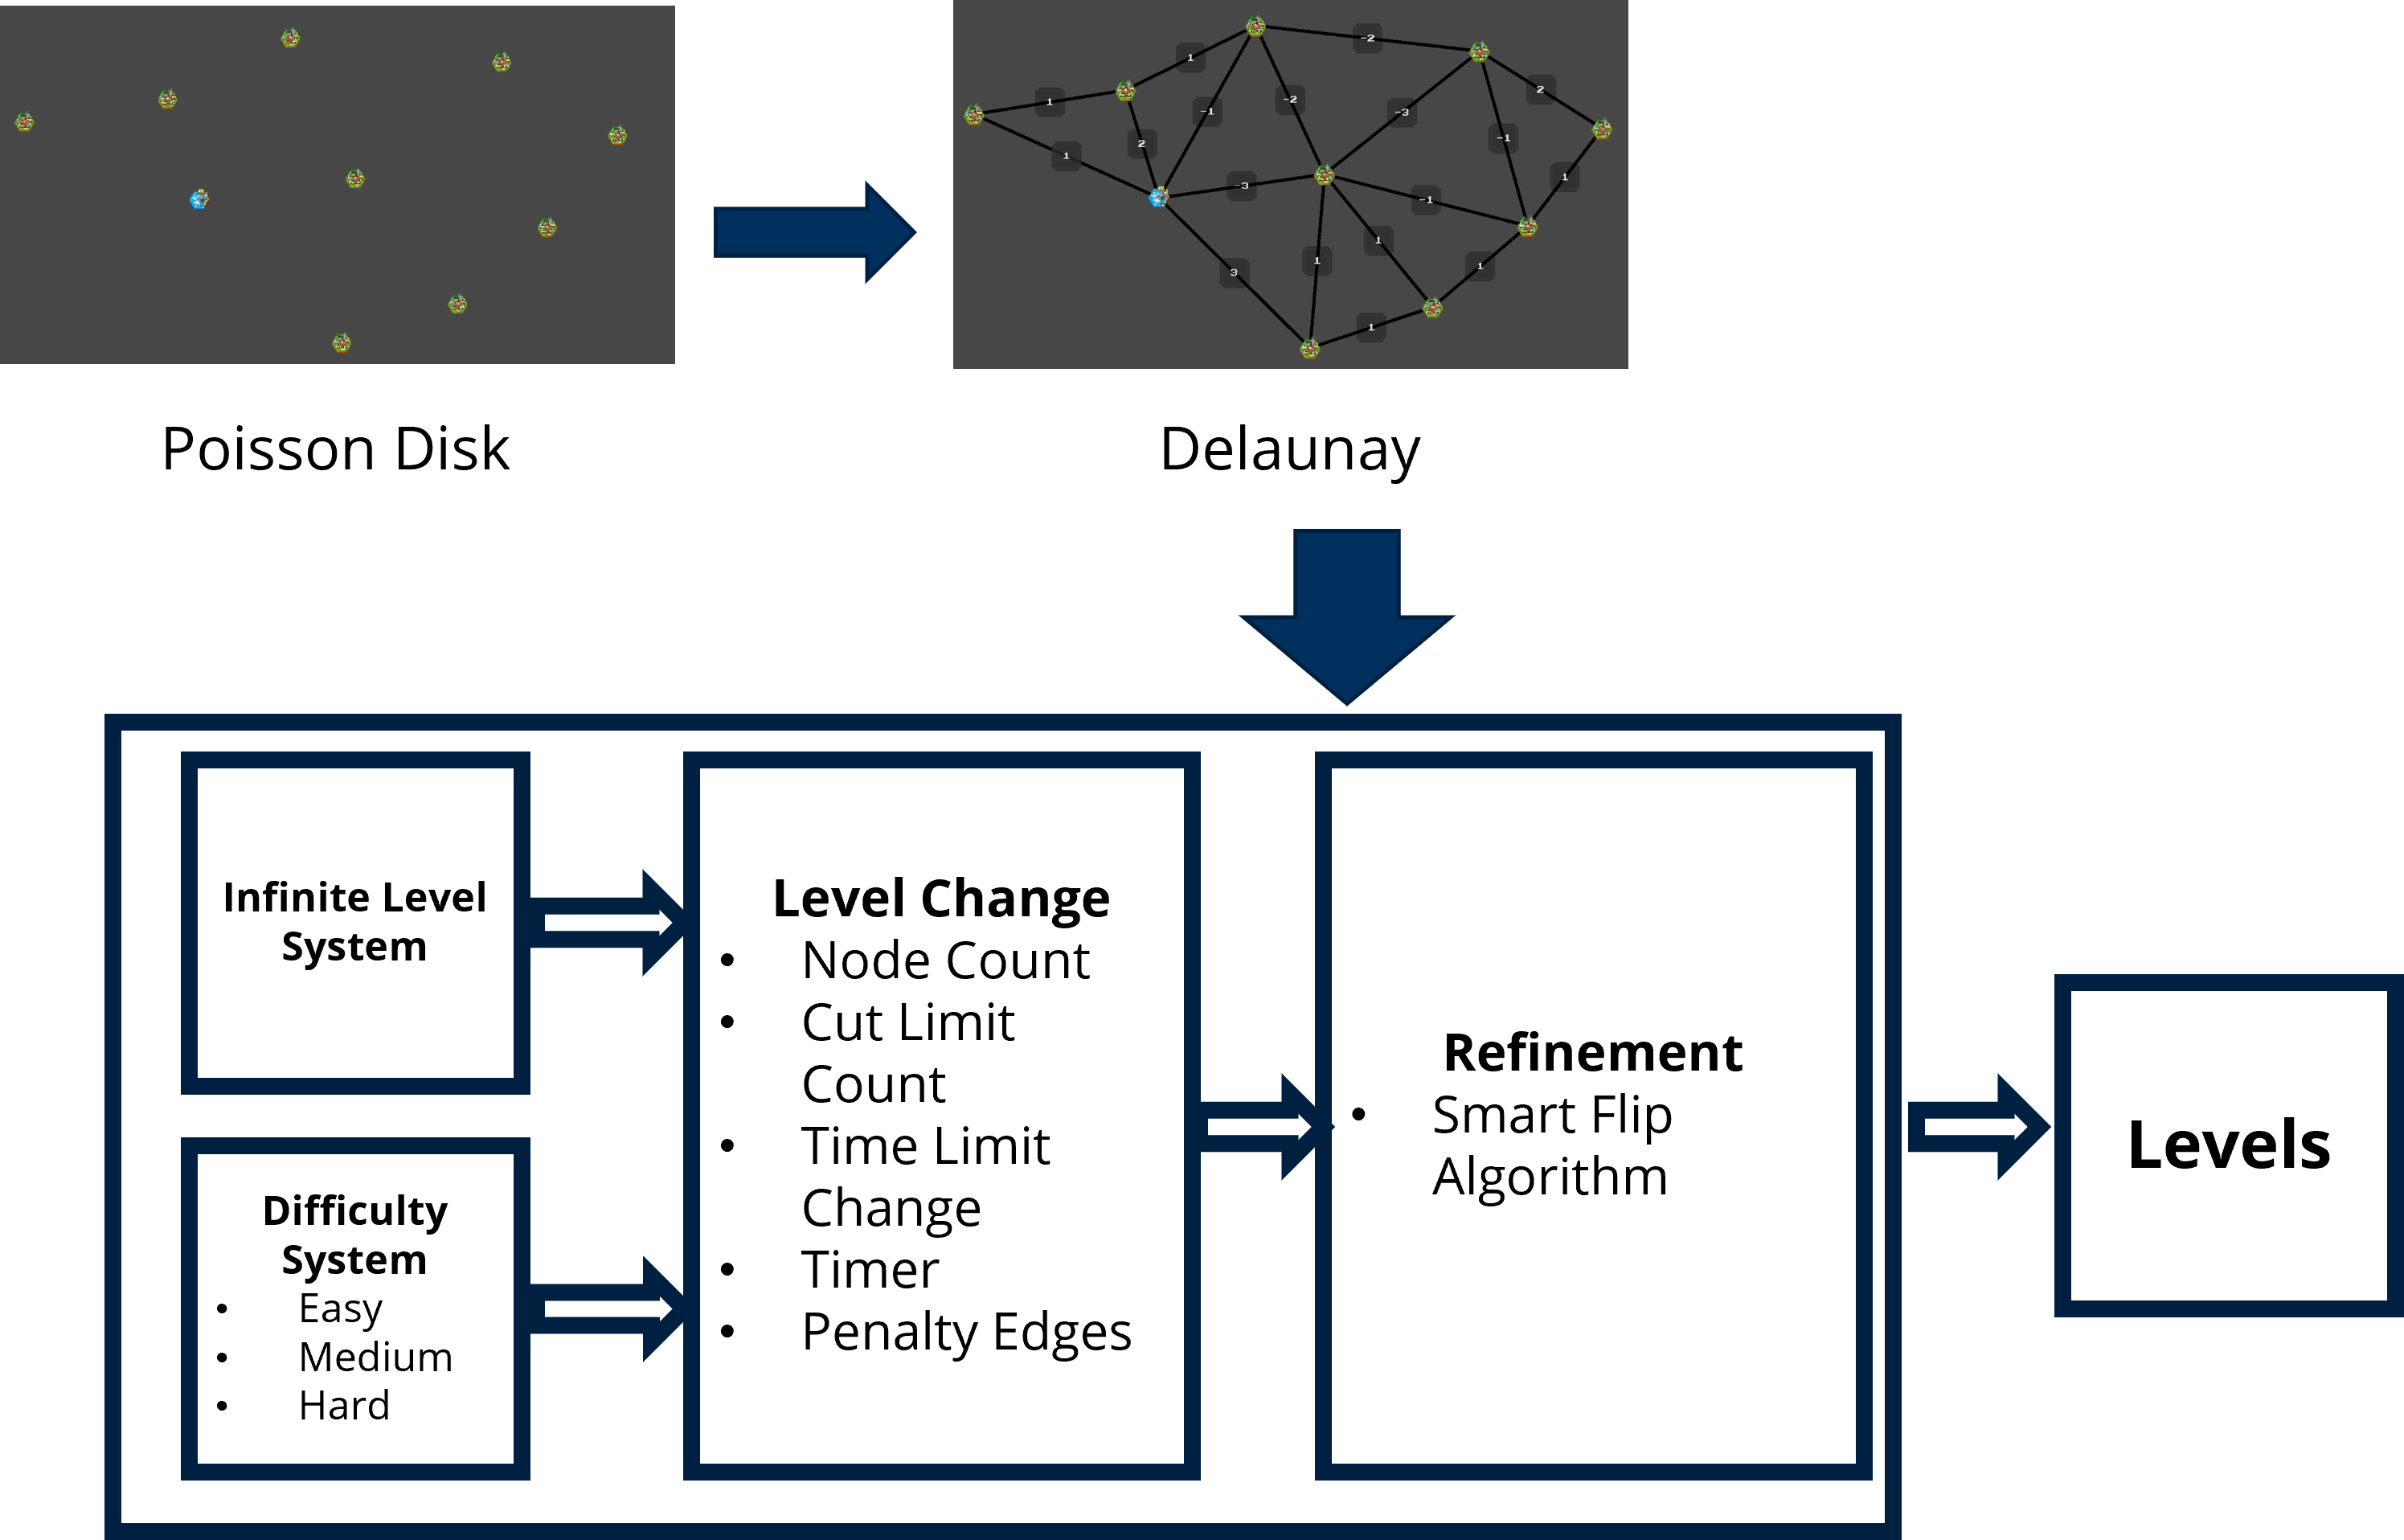
\includegraphics[width=0.8\textwidth]{figures/level_generation.png}
\caption{Level generation pipeline showing the complete process from node generation through Poisson disk sampling, Delaunay triangulation, weight calculation, and difficulty adjustment to final level validation.}
\label{fig:level_generation}
\end{figure}

\subsection{User Interface Design}
The main UI elements include COST display (current cost/optimal cost), level display (Level:Hard\_01), cut limit display (Cut Limit: 3/5), timer display, Hint Toggle button, territory Toggle button, victory panel, and menu return button. All UI components support automatic discovery and binding.

Game state information is displayed through real-time updated UI components. The system updates cost information, cut count, countdown, and level information automatically. The system uses coroutines and caching mechanisms to ensure responsive UI updates.

The hint system operates through Hint Toggle functionality. When activated, it calls the Python solver to obtain optimal cutting schemes and highlights edges that need to be cut using red highlight materials. The system supports dynamic highlighting/unhighlighting, with lines restoring correct rendering properties when Hint is deactivated. Hint functionality automatically deactivates during level transitions.

\subsection{Visual Design}
The game employs a medieval city-state themed pixel visual style. The hexagonal terrain system features unique colors and textures for different biomes. Edges display varying thickness and colors based on weight, with penalty edges shown in bold pink. Territory highlighting uses semi-transparent colors to distinguish different connected components.



\subsection{Alliance Territory Coloring}
The game employs a sophisticated and optimized territory coloring system that dynamically represents alliance clusters through efficient visual feedback mechanisms. This system is designed to provide immediate visual response to player actions while maintaining optimal performance through intelligent caching and selective updates.

\paragraph{Algorithm Foundation}
The territory coloring system is based on the \textbf{Nearest Neighbor Algorithm} to allocate terrain tiles to city-states. This algorithm ensures that each hexagonal tile is assigned to the closest city-state, creating natural-looking territory boundaries that reflect the current alliance structure.

\paragraph{Performance Optimization Strategy}
To minimize computational overhead and ensure smooth real-time performance, the system implements several optimization techniques:

\begin{itemize}
  \item \textbf{Selective Updates}: Only tiles affected by alliance changes are recalculated
  \item \textbf{Color Caching}: Pre-assigned colors are stored in a dictionary to avoid recalculation
  \item \textbf{Change Detection}: Efficient algorithms detect when clusters have actually changed
  \item \textbf{Batch Processing}: Multiple tile updates are processed in batches to reduce rendering overhead
\end{itemize}

\paragraph{Optimized Process Flow}
The enhanced coloring algorithm follows the optimized workflow illustrated in Figure~\ref{fig:territory_coloring_flowchart}. This flowchart demonstrates the complete process from edge cutting to selective visual updates, highlighting the key optimization strategies:

\begin{enumerate}
  \item \textbf{Edge Cut Detection}: Player cuts an edge, triggering the coloring update system
  \item \textbf{Cluster Change Analysis}: System analyzes if the cut actually changes any alliance clusters
    \begin{itemize}
      \item \textbf{No Change}: Skip visual update entirely, maintaining performance
      \item \textbf{Change Detected}: Proceed to selective tile identification
    \end{itemize}
  \item \textbf{Impact Zone Calculation}: Calculate only the tiles that need color updates
  \item \textbf{Color Assignment Optimization}: Check existing color assignments
    \begin{itemize}
      \item \textbf{Existing Colors}: Use cached colors for immediate updates
      \item \textbf{New Alliances}: Generate new colors only when necessary
    \end{itemize}
  \item \textbf{Selective Rendering}: Update only the affected tiles, not the entire map
\end{enumerate}

The flowchart clearly illustrates how the optimization system reduces computational overhead by implementing intelligent change detection and selective updates, ensuring that only necessary calculations are performed.

\paragraph{Technical Implementation Details}
The optimization system includes several key technical components:

\begin{itemize}
  \item \textbf{Distance Calculation Caching}: Pre-computed distances between tiles and city-states
  \item \textbf{Cluster State Tracking}: Efficient data structures to track alliance membership changes
  \item \textbf{Color Palette Management}: Optimized color assignment to minimize visual conflicts
  \item \textbf{Rendering Pipeline Integration}: Seamless integration with Unity's rendering system
\end{itemize}

\paragraph{Performance Benefits}
The optimized coloring system provides significant performance improvements:

\begin{itemize}
  \item \textbf{Reduced Computation}: 60-80\% reduction in unnecessary color calculations
  \item \textbf{Faster Response Time}: Immediate visual feedback for player actions
  \item \textbf{Lower Memory Usage}: Efficient caching reduces memory overhead
  \item \textbf{Scalability}: System maintains performance with larger maps and more city-states
\end{itemize}

This optimized system ensures that territory coloring dynamically reflects the current alliance structure while providing immediate visual feedback to players about the consequences of their strategic decisions, all while maintaining smooth performance across different hardware configurations.

\begin{figure}[h]
\centering
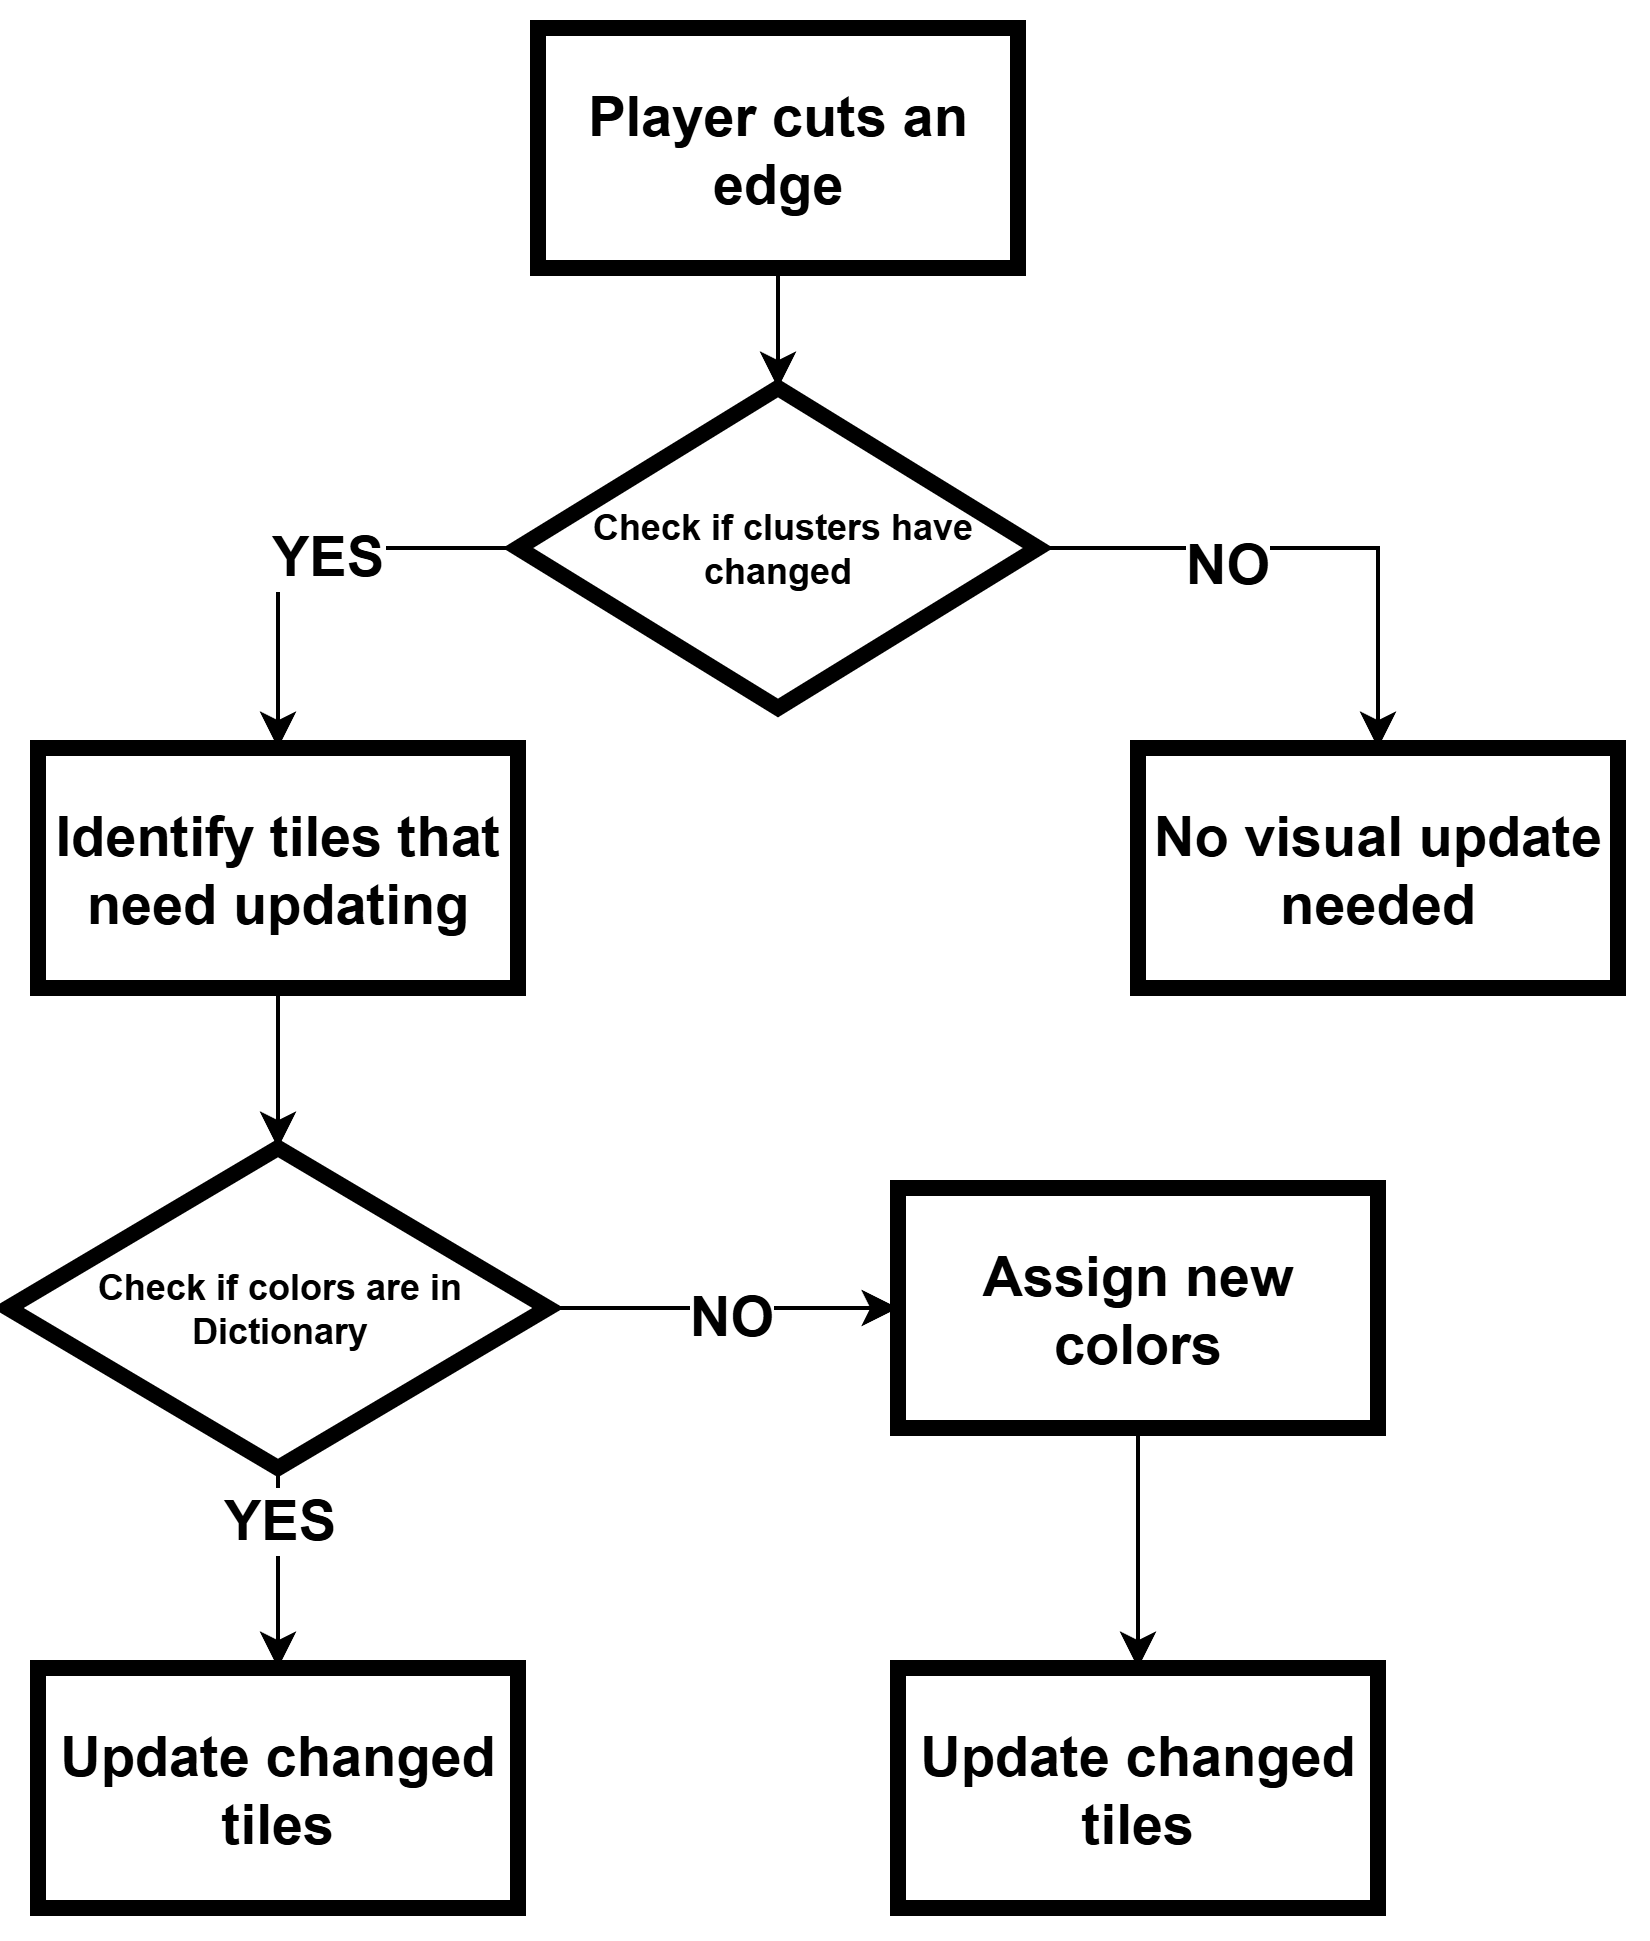
\includegraphics[width=0.6\textwidth]{figures/territory_coloring_flowchart.png}
\caption{Optimized territory coloring algorithm flowchart showing the performance-optimized workflow from edge cutting to selective visual updates, highlighting the caching mechanisms and change detection strategies that reduce computational overhead.}
\label{fig:territory_coloring_flowchart}
\end{figure}







\section{Future Prospects and Enhancements}

\subsection{Performance Optimization}
Future development will focus on optimizing territory display performance and resolving lag issues, implementing efficient rendering algorithms for large-scale maps, and enhancing real-time visual feedback systems to ensure smooth gameplay experience across different hardware configurations.

\subsection{Advanced Gameplay Features}
Planned advanced features include random events that introduce dynamic changes to edge weights during gameplay, hostile city-states that actively repair cut edges for confrontation, environmental factors such as mountains, rivers, and forests that modify edge weights, and multiplayer support for both collaborative and competitive gameplay modes.

\subsection{Educational Enhancements}
Educational enhancements will incorporate a comprehensive tutorial system with interactive learning modules for graph theory concepts, algorithmic problem generation for creating diverse problem instances, and an analytics dashboard providing detailed performance metrics and learning analytics to track educational effectiveness.

\section{Unresolved Questions and Future Work}
Several important questions remain to be addressed in future research and development. Performance scaling considerations include understanding how the game performs with very large graphs containing 100+ nodes, which is crucial for educational applications with complex scenarios. Educational effectiveness research is needed to quantify the learning impact compared to traditional teaching methods, providing empirical evidence for the game's pedagogical value. Accessibility improvements should explore how the game can be made more accessible to players with different learning styles and abilities. Finally, platform expansion feasibility studies should investigate the potential for developing mobile and web versions to increase accessibility and reach.

\section{Conclusion}

\subsection{Project Achievements}
The project successfully implemented an educational game "Alliance Divider" based on the Multicut Problem, achieving several significant accomplishments. The primary achievements include the complete implementation of a decoupled architecture between Unity and Python-Gurobi, resolving cross-platform compatibility issues; development of a comprehensive hexagonal terrain generation system including biome mapping and river generation; implementation of standard multicut algorithms with cycle inequality constraints; design of a progressive difficulty system incorporating innovative mechanisms such as time bombs; and creation of a territory visualization system that displays connected component changes in real-time.

The project successfully achieved its initial objectives by transforming the complex Multicut Problem into a playable game, making abstract graph theory concepts concrete through the medieval city-state alliance setting. The Unity-Python integration architecture resolved technical challenges in algorithmic solving, while the complete game system includes level generation, difficulty control, victory detection, and other essential functionalities. The project evolved from a simple prototype into a fully functional educational game.

\subsection{Technical Innovations}
The project introduced several technical breakthroughs and innovations. The Unity-Python file communication architecture avoided complex cross-platform integration issues, while Delaunay Refinement subdivision improved mesh quality. The terrain weight system associated terrain types with edge weights, and the time bomb trap mechanism increased strategic depth. The background calculation system enabled real-time territory updates, and reflection technology resolved system decoupling issues. These innovations enhanced system stability and user experience.

\subsection{Educational Value}
The project holds significant educational value by transforming abstract graph theory algorithms into intuitive gaming experiences, helping students understand the practical applications of the Multicut Problem. Through visual representation of algorithmic results, complex mathematical concepts become perceivable. Gamified learning increases student engagement and learning interest, transforming dry algorithmic learning into an engaging exploration process.

The game assists learning through multiple approaches: intuitive visualization of graph structures and cutting results; real-time feedback showing the gap between current and optimal solutions; interactive cutting mechanisms allowing players to experience algorithmic decision-making processes; territory highlighting helping understand connected component concepts; progressive difficulty systems adapting to different learning levels; and Hint systems providing learning guidance.

The project provides important insights for algorithmic education: gamification is an effective tool for algorithmic teaching; visualization significantly enhances understanding of abstract concepts; interactive experiences are more effective than passive learning; interdisciplinary background settings can enhance learning motivation; real-time feedback systems help consolidate concepts; and tiered difficulty design adapts to individual differences.

\subsection{Technical Contributions}
The project made contributions across multiple technical domains. The Unity-Python integration architecture provided new approaches for game development, while the file communication mechanism resolved cross-platform compatibility issues. The hexagonal terrain system demonstrated technical solutions for complex terrain generation, and the gamified implementation of multicut algorithms provided examples for algorithmic visualization. The real-time calculation system demonstrated optimization methods for background processing.

Integration experience includes: file communication being more stable and reliable than direct API calls; JSON format providing excellent data exchange standards; decoupled architecture facilitating maintenance and expansion; process management requiring proper handling of exceptions and timeouts; reflection technology resolving type reference limitations; and caching mechanisms improving performance.

\subsection{Limitations and Constraints}
The project faces several limitations. Game mechanics are relatively singular, lacking diverse gameplay options, while sound and music design remain incomplete. The project lacks detailed tutorials and documentation, and algorithm explanations are insufficiently deep, potentially affecting learning effectiveness. Performance optimization is limited, requiring high machine performance.

Technical constraints include: file communication mechanisms having delays affecting real-time performance; Python script dependencies on external environments complicating deployment; Unity version compatibility issues; memory usage efficiency requiring optimization; incomplete multi-threading processing; and relatively simple error recovery mechanisms.

Educational limitations include: lack of systematic learning path design; insufficiently detailed algorithm principle explanations; absence of tools for evaluating learning effectiveness; lack of personalized learning adaptation; incomplete learning progress tracking; and insufficient integration with other learning resources.

Game design shortcomings include: relatively singular gameplay lacking variation; absence of social and competitive elements; insufficient reward mechanisms; level design lacking narrative elements; user interface design requiring improvement; and absence of achievement systems.

\subsection{Future Development}
Future development directions include optimizing territory display performance and resolving lag issues, adding random events to change edge weights dynamically, implementing hostile city-states that actively repair cut edges for confrontation, and incorporating environmental factors such as mountains, rivers, and forests that modify edge weights. These enhancements would further improve the educational value and gameplay experience of the Alliance Divider game.

The Multicut Game project successfully demonstrates the potential of gamification in educational contexts, particularly for complex mathematical concepts. By combining Unity's powerful game engine with Python's optimization capabilities, the project creates an engaging platform for learning graph theory and combinatorial optimization. The modular architecture allows for future enhancements and scalability, making it a valuable tool for both education and research in algorithmic game theory.

\printbibliography[heading=bibintoc]\label{sec:bibliography}%

\end{document}

